% Options for packages loaded elsewhere
\PassOptionsToPackage{unicode}{hyperref}
\PassOptionsToPackage{hyphens}{url}
%
\documentclass[
  a4paper,
]{scrbook}

\usepackage{amsmath,amssymb}
\usepackage{lmodern}
\usepackage{iftex}
\ifPDFTeX
  \usepackage[T1]{fontenc}
  \usepackage[utf8]{inputenc}
  \usepackage{textcomp} % provide euro and other symbols
\else % if luatex or xetex
  \usepackage{unicode-math}
  \defaultfontfeatures{Scale=MatchLowercase}
  \defaultfontfeatures[\rmfamily]{Ligatures=TeX,Scale=1}
  \setmainfont[]{Latin Modern Roman}
  \setsansfont[]{Latin Modern Roman}
\fi
% Use upquote if available, for straight quotes in verbatim environments
\IfFileExists{upquote.sty}{\usepackage{upquote}}{}
\IfFileExists{microtype.sty}{% use microtype if available
  \usepackage[]{microtype}
  \UseMicrotypeSet[protrusion]{basicmath} % disable protrusion for tt fonts
}{}
\makeatletter
\@ifundefined{KOMAClassName}{% if non-KOMA class
  \IfFileExists{parskip.sty}{%
    \usepackage{parskip}
  }{% else
    \setlength{\parindent}{0pt}
    \setlength{\parskip}{6pt plus 2pt minus 1pt}}
}{% if KOMA class
  \KOMAoptions{parskip=half}}
\makeatother
\usepackage{xcolor}
\setlength{\emergencystretch}{3em} % prevent overfull lines
\setcounter{secnumdepth}{5}
% Make \paragraph and \subparagraph free-standing
\ifx\paragraph\undefined\else
  \let\oldparagraph\paragraph
  \renewcommand{\paragraph}[1]{\oldparagraph{#1}\mbox{}}
\fi
\ifx\subparagraph\undefined\else
  \let\oldsubparagraph\subparagraph
  \renewcommand{\subparagraph}[1]{\oldsubparagraph{#1}\mbox{}}
\fi


\providecommand{\tightlist}{%
  \setlength{\itemsep}{0pt}\setlength{\parskip}{0pt}}\usepackage{longtable,booktabs,array}
\usepackage{calc} % for calculating minipage widths
% Correct order of tables after \paragraph or \subparagraph
\usepackage{etoolbox}
\makeatletter
\patchcmd\longtable{\par}{\if@noskipsec\mbox{}\fi\par}{}{}
\makeatother
% Allow footnotes in longtable head/foot
\IfFileExists{footnotehyper.sty}{\usepackage{footnotehyper}}{\usepackage{footnote}}
\makesavenoteenv{longtable}
\usepackage{graphicx}
\makeatletter
\def\maxwidth{\ifdim\Gin@nat@width>\linewidth\linewidth\else\Gin@nat@width\fi}
\def\maxheight{\ifdim\Gin@nat@height>\textheight\textheight\else\Gin@nat@height\fi}
\makeatother
% Scale images if necessary, so that they will not overflow the page
% margins by default, and it is still possible to overwrite the defaults
% using explicit options in \includegraphics[width, height, ...]{}
\setkeys{Gin}{width=\maxwidth,height=\maxheight,keepaspectratio}
% Set default figure placement to htbp
\makeatletter
\def\fps@figure{htbp}
\makeatother

\usepackage{titling}
\setlength{\droptitle}{-2cm}
\preauthor{
  \begin{center}
  \Large
  \vspace{10mm}
  by

  \vspace{20mm}
}
\postauthor{
  \end{center}
  \vfill
}

\predate{
  \begin{center}
  A thesis 
  submitted in fulfilment of the \\
  requirements of the degree of \\
  Doctor of Philosophy in Physics\\               % Degree
  School of Physical and Chemical Sciences\\          % Department
  Te Herenga Waka - Victoria University of Wellington\\                       % University 
  \vspace{5mm}
}
\postdate{
  \\
  
\includegraphics[width=3in,height=1.5in]{figures/VUW-logo.png}\\
  \end{center}
  }
\makeatletter
\makeatother
\makeatletter
\@ifpackageloaded{bookmark}{}{\usepackage{bookmark}}
\makeatother
\makeatletter
\@ifpackageloaded{caption}{}{\usepackage{caption}}
\AtBeginDocument{%
\ifdefined\contentsname
  \renewcommand*\contentsname{Table of contents}
\else
  \newcommand\contentsname{Table of contents}
\fi
\ifdefined\listfigurename
  \renewcommand*\listfigurename{List of Figures}
\else
  \newcommand\listfigurename{List of Figures}
\fi
\ifdefined\listtablename
  \renewcommand*\listtablename{List of Tables}
\else
  \newcommand\listtablename{List of Tables}
\fi
\ifdefined\figurename
  \renewcommand*\figurename{Figure}
\else
  \newcommand\figurename{Figure}
\fi
\ifdefined\tablename
  \renewcommand*\tablename{Table}
\else
  \newcommand\tablename{Table}
\fi
}
\@ifpackageloaded{float}{}{\usepackage{float}}
\floatstyle{ruled}
\@ifundefined{c@chapter}{\newfloat{codelisting}{h}{lop}}{\newfloat{codelisting}{h}{lop}[chapter]}
\floatname{codelisting}{Listing}
\newcommand*\listoflistings{\listof{codelisting}{List of Listings}}
\makeatother
\makeatletter
\@ifpackageloaded{caption}{}{\usepackage{caption}}
\@ifpackageloaded{subcaption}{}{\usepackage{subcaption}}
\makeatother
\makeatletter
\@ifpackageloaded{tcolorbox}{}{\usepackage[many]{tcolorbox}}
\makeatother
\makeatletter
\@ifundefined{shadecolor}{\definecolor{shadecolor}{rgb}{.97, .97, .97}}
\makeatother
\makeatletter
\makeatother
\ifLuaTeX
  \usepackage{selnolig}  % disable illegal ligatures
\fi
\usepackage[citestyle = ieee,urldate = iso8601]{biblatex}
\addbibresource{references.bib}
\IfFileExists{bookmark.sty}{\usepackage{bookmark}}{\usepackage{hyperref}}
\IfFileExists{xurl.sty}{\usepackage{xurl}}{} % add URL line breaks if available
\urlstyle{same} % disable monospaced font for URLs
\hypersetup{
  pdftitle={Volatile Organic Compound Detection Using Insect Odorant-Receptor Functionalised Field-Effect Transistors},
  pdfauthor={Eddyn Oswald Perkins Treacher},
  hidelinks,
  pdfcreator={LaTeX via pandoc}}

\title{Volatile Organic Compound Detection Using Insect Odorant-Receptor
Functionalised Field-Effect Transistors}
\author{Eddyn Oswald Perkins Treacher}
\date{Oct 2023}

\begin{document}
\frontmatter
\maketitle
\ifdefined\Shaded\renewenvironment{Shaded}{\begin{tcolorbox}[boxrule=0pt, breakable, enhanced, borderline west={3pt}{0pt}{shadecolor}, sharp corners, frame hidden, interior hidden]}{\end{tcolorbox}}\fi

\mainmatter
\bookmarksetup{startatroot}

\hypertarget{acknowledgements}{%
\chapter*{Acknowledgements}\label{acknowledgements}}
\addcontentsline{toc}{chapter}{Acknowledgements}

\markboth{Acknowledgements}{Acknowledgements}

\begin{verbatim}
69450
\end{verbatim}

Rifat, Alex - vapour sensor Erica Cassie - FET sensing setup Rob Keyzers
and Jennie Ramirez-Garcia - NMR spectra Patricia Hunt - Computational
chemistry

\bookmarksetup{startatroot}

\hypertarget{verifying-non-covalent-functionalisation-of-carbon-nanotubes-and-graphene}{%
\chapter{Verifying Non-Covalent Functionalisation of Carbon Nanotubes
and
Graphene}\label{verifying-non-covalent-functionalisation-of-carbon-nanotubes-and-graphene}}

\begin{verbatim}
252732
\end{verbatim}

In previous chapters, we have discussed methods of fabricating carbon
nanotube and graphene devices and then shown that they can be operated
effectively as chemical sensors. However, to detect specific chemical
traces while ignoring others (`specific sensing'), the devices require
chemical modification, often called `functionalisation'. Instead of
responding to stimuli themselves, the sensing signal is picked up by
attached receptors. The devices then act as passive transducers for the
received signal. Receptors previously used with carbon nanotube and
graphene devices include aptamers and a range of proteins, including
odorant receptors. A common approach to attaching receptors to the
transducer involves the use of a linker molecule to tether the receptor
to the transducer. Verifying that this linker molecule is bridging
between the transducer and the receptor element is important for a
complete understanding of the behaviour of these sensors. This
verification involves providing evidence for effective attachment of
linker molecule to the transducing device channel, then showing
successful tethering of odorant receptors and other biomolecules to the
attached linker molecule.

This chapter therefore takes some time to explore the attachment of
linker molecules to carbon nanotube and graphene device channels, using
methods such as Raman spectroscopy, fluorescence microscopy and
electrical characterisation. Linker molecules used are discussed in
detail, and numerous hurdles to successful functionalisation via linker
molecules are identified and addressed.

\hypertarget{non-covalent-functionalisation-linker-molecules}{%
\section{Non-Covalent Functionalisation \& Linker
Molecules}\label{non-covalent-functionalisation-linker-molecules}}

Linker molecules may be attached via covalent or non-covalent bonding to
carbon nanomaterials, such as carbon nanotubes and graphene.
Non-covalent bonding is weaker and therefore less stable than covalent
bonding. However, non-covalent bonding has the advantage of having less
of an impact on the structure of a nanomaterial than covalent bonding,
and therefore is less likely to negatively affect the electrical
properties of the transducer
\autocite{Long2012,DiCrescenzo2014,Wang2020,Mishyn2022}. For example,
one group found covalent bonding of diazonium linker caused a
\(\sim 50\)\% drop in graphene channel mobility \autocite{Lerner2014}.
In comparison, only a \(\sim 5\)\% drop in mobility was seen for
attachment of a mixture of linkers containing pyrene to a graphene
channel via non-covalent \(\pi\) stacking \autocite{Thodkar2021}.

\(\pi\) stacking or \(\pi-\pi\) interaction is often used to describe a
type of non-covalent bonding which occurs due to dispersion forces
between unsaturated polycyclic molecules \autocite{Perez2015}. It has
been argued that this label is unhelpfully specific and a
misrepresentation of what can be simply classed as a type of Van Der
Waals bonding \autocite{Martinez2012,Perez2015}. However, as the use of
the term is widespread in the literature, it is also used here for ease
of reference. Carbon nanotubes and graphene consist of a network of
carbon atoms attached to each other by sp\(^{2}\) hybrid orbitals in a
polycyclic structure. They are therefore able to strongly interact with
linker molecules with aromatic moieties, such as pyrene
\autocite{Hermanson2013-16,Perez2015,Mishyn2022}.
Figure~\ref{fig-pi-interaction-cnt} is a visual demonstration of the
relationship between the pyrene-based linker molecule with the
transducer and receptor elements. \(\pi-\pi\) stacking with pyrene is
the bonding mechanism underlying all the functionalisation processes in
this thesis.

\begin{figure}

{\centering 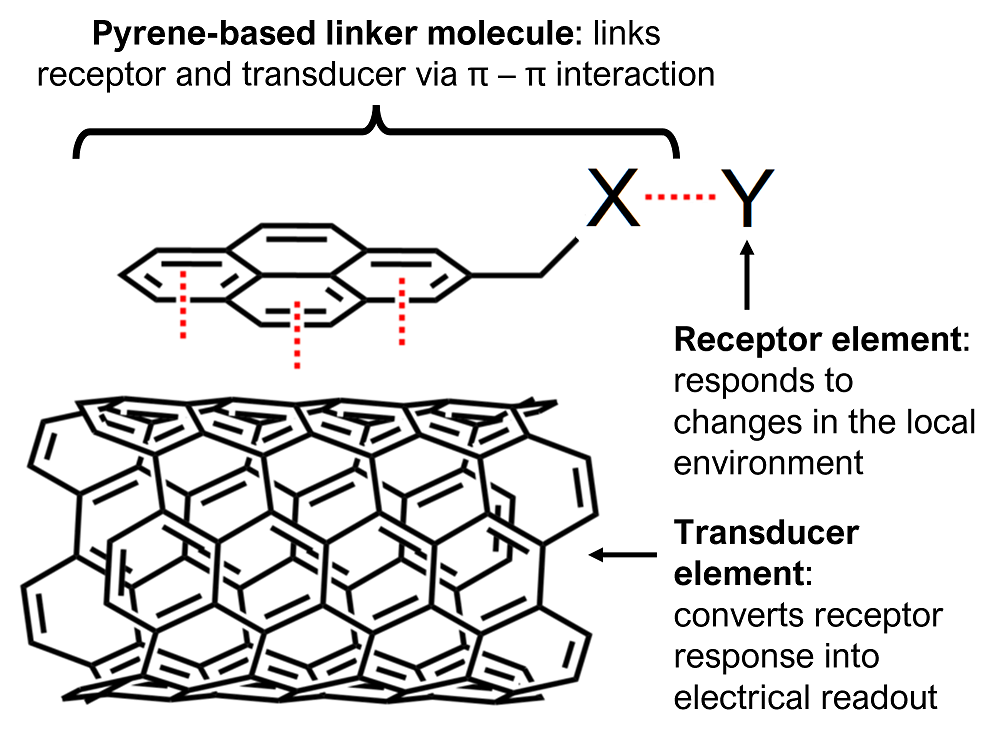
\includegraphics[width=0.8\textwidth,height=\textheight]{./figures/ch6/pyrene-cnt.png}

}

\caption{\label{fig-pi-interaction-cnt}Attachment of pyrene-based linker
molecule pyrene-X and receptor Y to a carbon nanotube, representing the
transducer element of a field-effect transistor. Source: Adapted from
\autocite{Carbonnanotube}.}

\end{figure}

\newpage
\KOMAoptions{paper=landscape,pagesize}

\hypertarget{tbl-pbase-functionalisation}{}
\begin{longtable}[]{@{}lllllll@{}}
\caption{\label{tbl-pbase-functionalisation}Comparison of PBASE
functionalisation processes used for immobilisation of proteins and
aptamers onto carbon nanotubes and graphene. Experimentally optimised
variables are marked with a star (*). Blank entries indicate there was
no mention of the parameter in a particular paper.}\tabularnewline
\toprule()
Solvent & Channel & Conc. (mM) & Incubation type & Time (hr) & Rinse
steps & References \\
\midrule()
\endfirsthead
\toprule()
Solvent & Channel & Conc. (mM) & Incubation type & Time (hr) & Rinse
steps & References \\
\midrule()
\endhead
DMF & CNT & 5 & Immersed & 1 & PBS & Maehashi \textit{et al.}
\cite{Maehashi2007} \\
& & 6 & Immersed & 1 & DMF, PBS & García-Aljaro \textit{et al.}
\cite{Garcia-Aljaro2010} \\
& & 6 & Immersed & 1 & DMF & Chen \textit{et al.} \cite{Chen2001} \\
& & 6 & Immersed & 1 & DMF & Cella \textit{et al.} \cite{Cella2010} \\
& & 6 & Immersed & 1 & DMF & Das \textit{et al.} \cite{Das2011} \\
& & 6 & - & 2 & DMF & Besteman \textit {et al.} \cite{Besteman2003} \\
& Graphene & - & - & 2 & DMF & Kwong Hong Tsang \textit{et al.}
\cite{KwongHongTsang2019} \\
& & - & - & 20 & - & Wiedman \textit{et al.} \cite{Wiedman2017} \\
& & 0.2 & Immersed & 20 & DMF, IPA, DI water & Gao \textit{et al.}
\cite{Gao2018} \\
& & 1 & 100 \(\mu\)L droplet & 6 & DMF, IPA, DI water & Nekrasov
\textit{et al.} \cite{Nekrasov2021} \\
& & 5 & Immersed & 1 & DMF, DI water & Hwang \textit{et al.}
\cite{Hwang2016} \\
& & 5* & Immersed & 3* & DMF & Hao \textit{et al.} \cite{Hao2020} \\
& & 5 & Immersed, with agitation & 4* & DMF, DI water & Mishyn
\textit{et al.} \cite{Mishyn2022} \\
& & 6 & 6 \(\mu\)L droplet & 2 & DMF, DI water & Nur Nasufiya
\textit{et al.} \cite{NurNasyifa2020} \\
& & 10 & 10 \(\mu\)L droplet & 2 & DMF, DI water & Campos
\textit{et al.} \cite{Campos2019} \\
& & 10 & Immersed & 2 & DMF, PBS & Kuscu \textit{et al.}
\cite{Kuscu2020} \\
& & 10 & Immersed & 1 & DMF & Xu \textit{et al.} \cite{Xu2017} \\
& & 10 & Immersed & 12 & DMF, ethanol, DI water & Khan \textit{et al.}
\cite{Khan2020} \\
& & 50 & Immersed & 4* & Methanol & Wang \textit{et al.}
\cite{Wang2020} \\
2-Methoxyethanol & Graphene & 1 & Immersed & 1 & DI water & Ono
\textit{et al.} \cite{Ono2020} \\
Methanol & CNT & 1 & Immersed & 1 & Methanol, DI water & Zheng
\textit{et al.} \cite{Zheng2016} \\
& & 1 & Immersed & 2 & Methanol & Kim \textit{et al.} \cite{Kim2009} \\
& & 100 & 2 \(\mu\)L droplet & 1 & DI water & Yoo \textit{et al.}
\cite{Yoo2022} \\
& Graphene & 5 & Immersed & 2 & - & Sethi \textit{et al.}
\cite{Sethi2020} \\
& & 5 & Immersed & 1 & Methanol, PBS & Ohno \textit{et al.}
\cite{Ohno2010} \\
DMSO & CNT & 10 & - & 1 & DI water & Lopez \textit{et al.}
\cite{Lopez2015} \\
& & 10 & Immersed & 1 & PBS & Strack \textit{et al.}
\cite{Strack2013} \\
\bottomrule()
\end{longtable}

\newpage
\KOMAoptions{paper=portrait,pagesize}

\hypertarget{sec-PBASE}{%
\subsection{1-Pyrenebutanoic acid N-hydroxysuccinimide ester
(PBASE)}\label{sec-PBASE}}

\begin{figure}

\begin{minipage}[t]{0.47\linewidth}

{\centering 

\raisebox{-\height}{

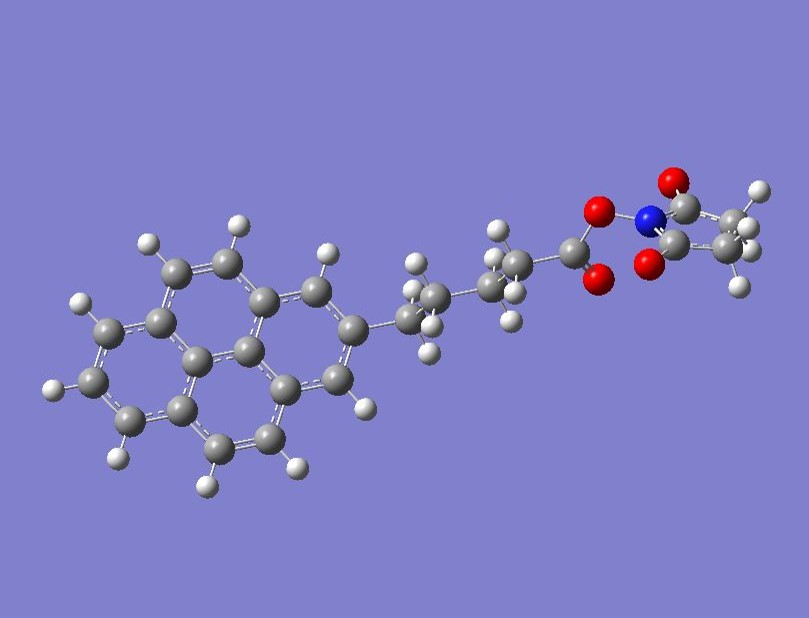
\includegraphics{./figures/ch6/pbase_stable_1.png}

}

}

\subcaption{\label{fig-pbase-stable-1}}
\end{minipage}%
%
\begin{minipage}[t]{0.05\linewidth}

{\centering 

~

}

\end{minipage}%
%
\begin{minipage}[t]{0.47\linewidth}

{\centering 

\raisebox{-\height}{

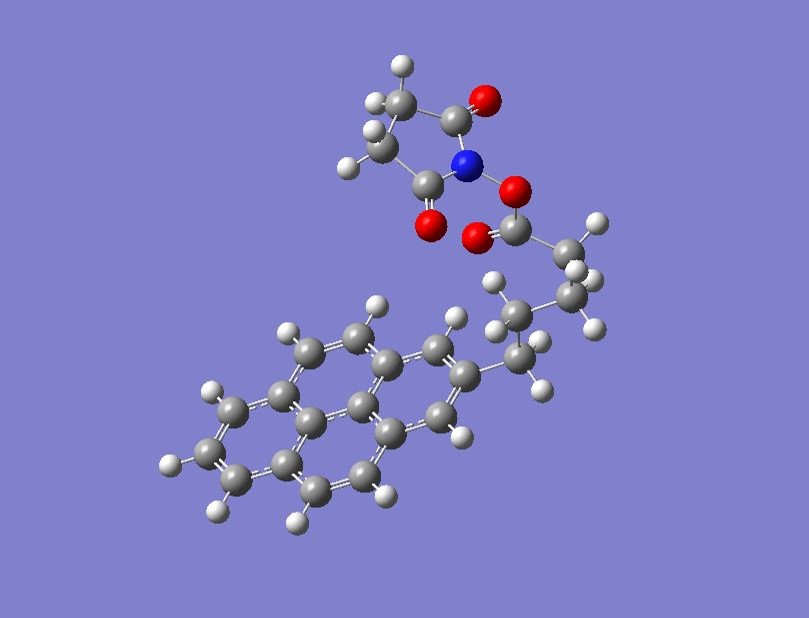
\includegraphics{./figures/ch6/pbase_stable_2.png}

}

}

\subcaption{\label{fig-pbase-stable-2}}
\end{minipage}%

\caption{\label{fig-pbase-structure}Two conformations of PBASE molecule
with geometry optimised via \emph{ab initio} calculations (computed
using Gaussian 16 \autocite{g16}). White balls correspond to hydrogen,
grey to carbon, red to oxygen and blue to nitrogen. The conformation in
(a) has a Hartree-Fock energy of -3427728.67 kJ/mol, while the
conformation in (b) has a Hartree-Fock energy of -3427729.66 kJ/mol. The
difference between computed Hartree-Fock energies is 1.0 kJ/mol, small
enough that the existence of both molecular conformations is physically
feasible.}

\end{figure}

1-Pyrenebutanoic acid N-hydroxysuccinimide ester (variously known
commercially and in the literature as 1-Pyrenebutyric acid
N-hydroxysuccinimide ester, PBASE, PBSE, PASE, Pyr-NHS, PyBASE, PANHS)
is a aromatic, bifunctional molecule commonly used for tethering
biomolecules to the carbon rings of graphene and carbon nanotubes. The
molecular structure of PBASE is shown in
Figure~\ref{fig-pbase-structure}. Two locally stable molecular
conformations were found to exist, a straight
(Figure~\ref{fig-pbase-stable-1}) and bent
(Figure~\ref{fig-pbase-stable-2}) structure. Similar locally stable
structures have previously been computed for PBASE attached to graphene
\autocite{Oishi2022}. The pyrene moiety, seen at the bottom of the
molecular structure, non-covalently bonds to the carbon rings of the
carbon nanotube and graphene surface. An N-hydroxysuccinimide (NHS)
ester group is found at the top of the molecular structure, attached to
the rest of the molecule via a O-C bond. The NHS ester group is highly
reactive with amine groups; it can undergo a nucleophilic substitution
reaction with amines attached to proteins or aptamers, tethering these
biomolecules via an amide or imide bond
\autocite{Chen2001,Hermanson2013-16,Hermanson2013-3,Mishyn2022}.

The non-covalent functionalisation of proteins onto a single-walled
carbon nanotube using PBASE was first reported by Chen \emph{et al.} in
2001 \autocite{Chen2001}. Two methods for protein functionalisation and
immobilisation were successfully used, with the only differences being
the solvent used to dissolve the PBASE powder (DMF, methanol) and the
final concentration of the resulting solutions (6 mM, 1 mM
respectively). The lower concentration may have been used for PBASE in
methanol as PBASE powder appears to dissolve poorly in methanol at
higher concentrations. Several groups directly cite Chen \emph{et al.}
when discussing functionalisation with PBASE
\autocite{Besteman2003,Cella2010,Campos2019,Zheng2016,Ohno2010}. Other
groups using PBASE for graphene or carbon nanotube functionalisation do
not explicitly reference Chen \emph{et al.} in their methodology, but it
is apparent they often draw on one of these two original methods. This
common ancestry becomes apparent from the high frequency of methods
detailing the use of 6 mM PBASE in dimethylformamide (DMF) and 1 mM
PBASE in methanol, as seen in Table~\ref{tbl-pbase-functionalisation}.

\begin{figure}

\begin{minipage}[t]{\linewidth}

{\centering 

\raisebox{-\height}{

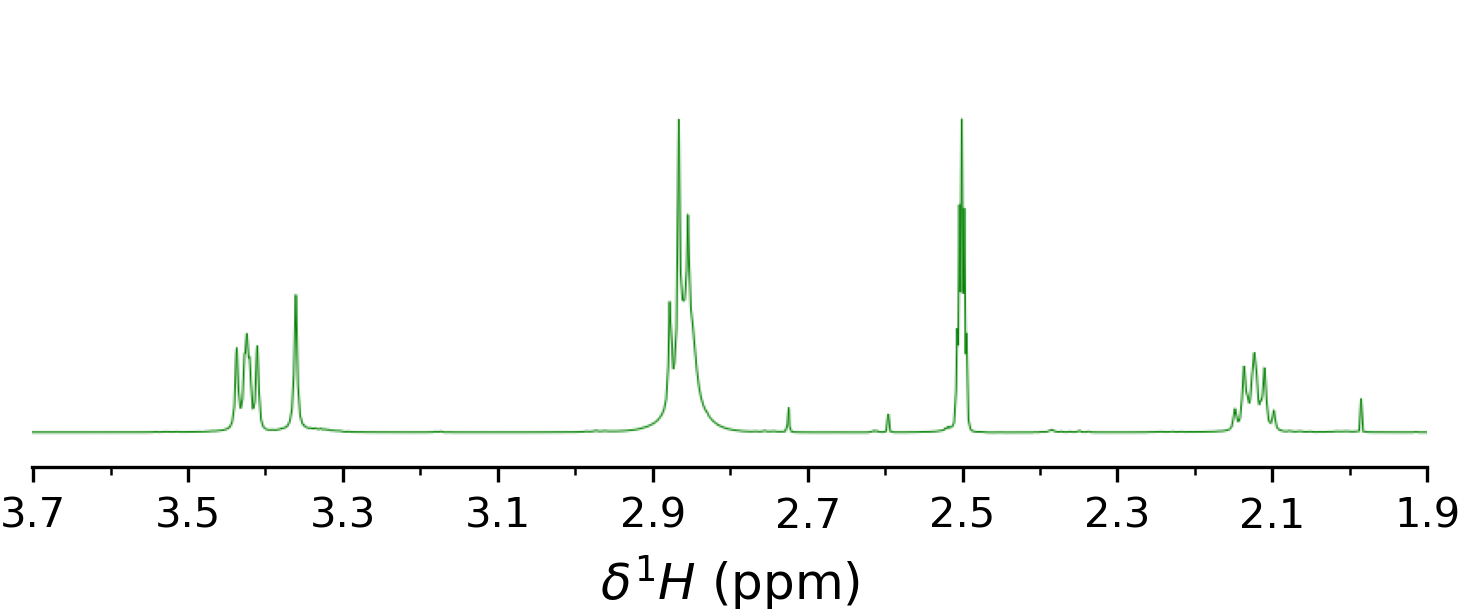
\includegraphics{./figures/ch6/modified_sigma_pbase_nmr.png}

}

}

\subcaption{\label{fig-sigma-nmr}}
\end{minipage}%
\newline
\begin{minipage}[t]{\linewidth}

{\centering 

\raisebox{-\height}{

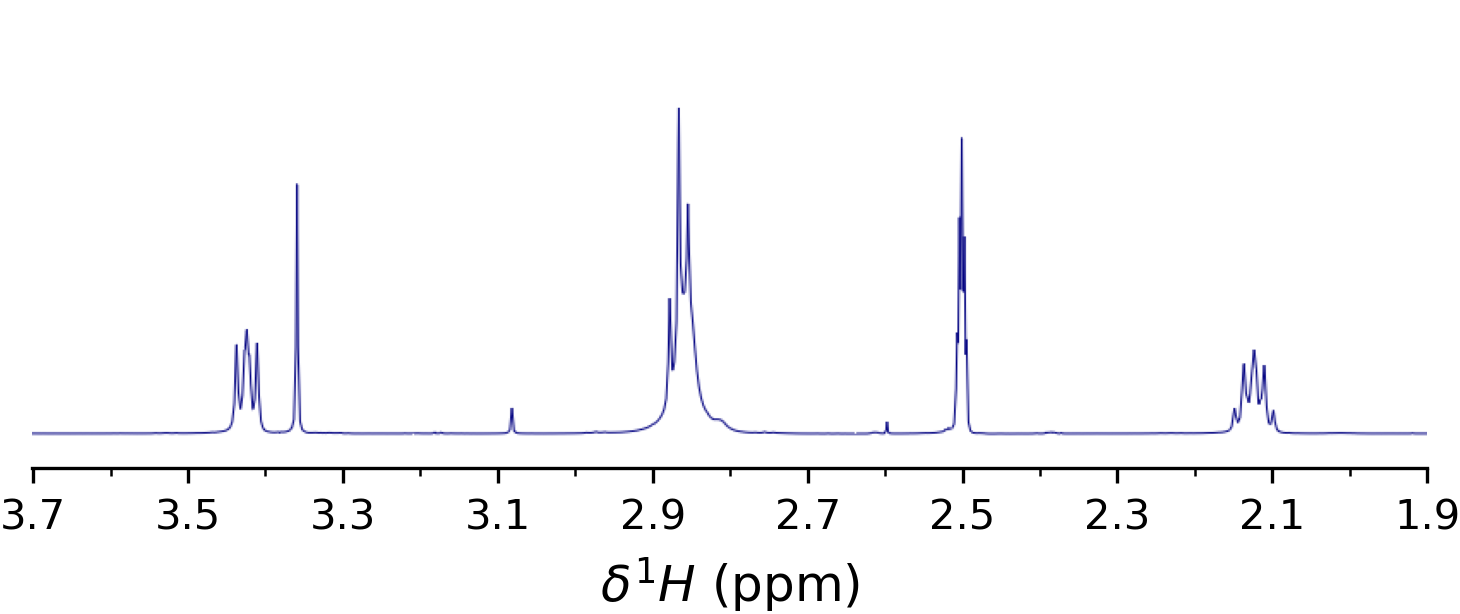
\includegraphics{./figures/ch6/modified_setareh_pbase_nmr.png}

}

}

\subcaption{\label{fig-setareh-nmr}}
\end{minipage}%
\newline
\begin{minipage}[t]{\linewidth}

{\centering 

\raisebox{-\height}{

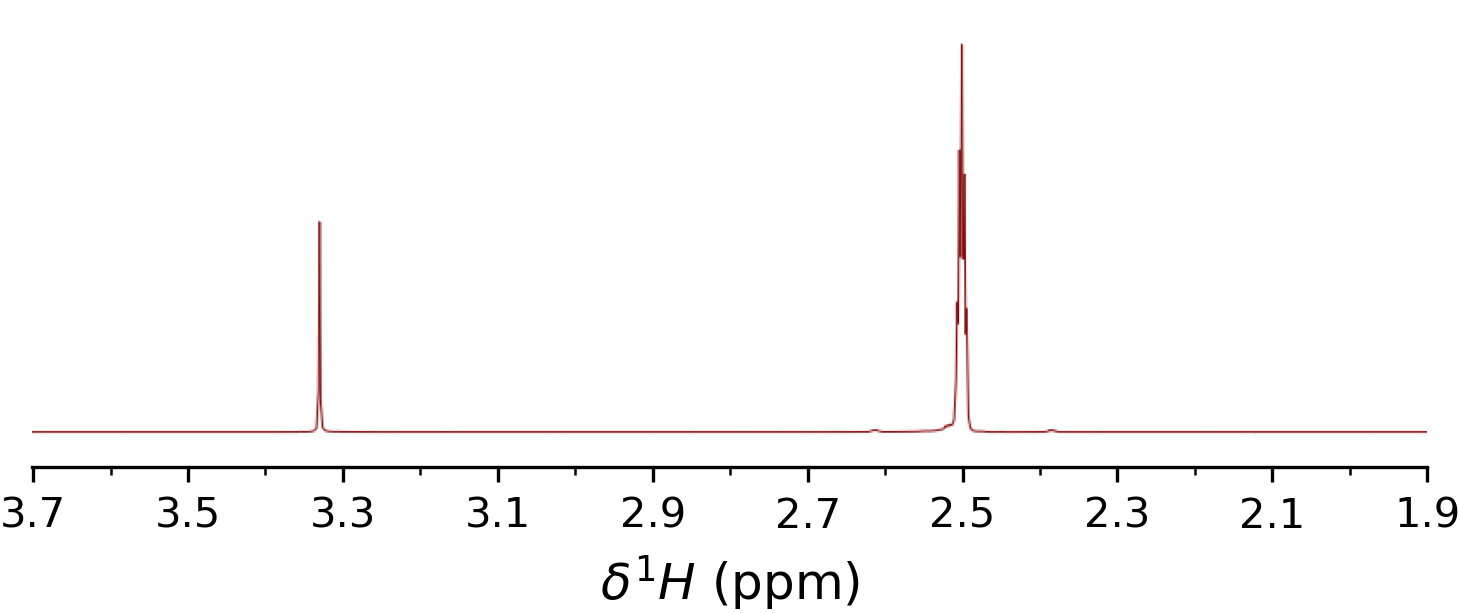
\includegraphics{./figures/ch6/modified_dmso_nmr.png}

}

}

\subcaption{\label{fig-dmso-nmr}}
\end{minipage}%

\caption{\label{fig-pbase-nmr}\(^{1}\)H Nuclear Magnetic Resonance (NMR)
spectra, performed with DMSO-d\(_6\) used as the NMR solvent. (a) and
(b) show NMR spectrum for commercially purchased PBASE, from
Sigma-Aldrich and Setareh Biotech respectively, while (c) shows the
blank spectrum taken with only DMSO-d\(_6\) present (spectra taken by
Jennie Ramirez-Garcia).}

\end{figure}

However, it is also apparent from
Table~\ref{tbl-pbase-functionalisation} that there is a large degree of
variation in the methods used for PBASE functionalisation. Various
electrical characterisation, microscopy and spectroscopy techniques have
been used to demonstrate successful functionalisation. Until recently,
there has been little justification provided for the selection of
variables used in the functionalisation procedure (e.g.~length of time
submerged in solvent containing PBASE), despite the wide-ranging use of
this process in the literature \autocite{Hinnemo2017,Zhen2018,Wang2020}.
This is surprising, given that the sensitivity of functionalised devices
is considered to be closely related to the density of surface
functionalisation \autocite{White2008,Hermanson2013-3,Chen2014}.
Furthermore, a detailed investigation of PBASE functionalisation process
variables has only been undertaken for graphene-based devices
\autocite{Zhen2018,Hao2020,Wang2020,Mishyn2022}.

Zhen \emph{et al.}, Wang \emph{et al.} and Mishyn \emph{et al.} claim
that carefully tuning the surface concentration of PBASE is required to
avoid multilayer coverage of the graphene surface, as this negatively
impacts sensing. Mishyn \emph{et al.} use cyclic voltammetry to
demonstrate that less receptor attachment to the graphene surface occurs
when multiple layers of PBASE are present. However, neither group lends
further support to their claim by performing analyte sensing using their
functionalised graphene devices \autocite{Zhen2018,Mishyn2022}. In
contrast, Hao \emph{et al.} find that maximising surface coverage of
PBASE results in more sensitive aptameric sensing, thus drawing the
opposite conclusion \autocite{Hao2020}. The inconsistency in these
recent findings mean more work is needed to understand the PBASE
functionalisation process to achieve optimal biosensor sensitivity. It
may also be the case that a specific functionalisation process is
required for optimal sensitivity with the use of a specific type of
receptor.

Once fastened to a bioreceptor via an amide or imide bond, the
attachment to the linker molecule is not easily broken. However, prior
to use in functionalisation processes, the NHS ester may react with any
water present (hydrolysis). This reaction converts PBASE to
1-pyrenebutyric acid (PBA), leaving it unavailable to react further with
amine groups \autocite{Hermanson2013-3,Hermanson2013-5,Mishyn2022}. If
the amine group functionalisation is performed within a \$\sim\$1 hour
period, with a high concentration of bioreceptor used at close to
neutral pH, competing hydrolysis should not have a significantly adverse
impact on the functionalisation process \autocite{Hermanson2013-3}.
However, if PBASE is exposed to water during storage over a significant
length of time, the presence of
1-Ethyl-3-(3-dimethylaminopropyl)carbodiimide (EDC) can be used to
restore the NHS ester and enable the substitution reaction to take place
(see discussion of PBA/EDC in Section~\ref{sec-other-linkers}).

We purchased PBASE from two suppliers, Sigma-Aldrich and Setareh
Biotech. Sigma recommended DMF and methanol as suitable solvents for
dissolving PBASE, alongside chloroform and dimethyl sulfoxide (DMSO).
Setareh Biotech indicated methanol can be used for dissolving PBASE. The
two suppliers had conflicting information for suitable storage of PBASE,
with Sigma recommending room temperature storage while Setareh Biotech
recommends storage of \(-5\) to \(-30 ^\circ \text{C}\) and protection
from light and moisture. Given the long travel time of the PBASE samples
under uncertain storage conditions, we used nuclear magnetic resonance
(NMR) spectroscopy to verify the purity of the PBASE as recieved from
each supplier. In light of the negative effect of water on PBASE, in
particular we wanted to find out if any water was present in the
samples.

Figure~\ref{fig-pbase-nmr} compares the shapes of hydrogen (NMR) spectra
of PBASE from each supplier when dissolved in deuterated DMSO, alongside
a blank deuterated DMSO spectrum. We see both PBASE samples possess
characteristic chemical shift features between \(2.1-2.2\) ppm,
\(2.8-2.9\) ppm, and \(3.4-3.5\) ppm. These chemical shifts roughly
correspond to those seen in previous NMR spectra for PBASE
\autocite{NMR2}. The feature at 2.50 ppm represents the deuterated DMSO
solvent, while the single peak between \(3.3-3.4\) ppm represents the
water present in the sample. By comparing the area of these peaks, we
can estimate the amount of water originally present in the PBASE sample.
The H\(_{2}\)O:DMSO ratio is 1:7 in the blank spectrum, but \(\sim\) 1:3
in the provided samples, possibly indicating the introduction of water
to the PBASE during production or storage. However, DMSO is strongly
hygroscopic and slight differences in DMSO storage time, as well as
differences in humidity during sample preparation, may have had a
significant impact on this result \autocite{Lebel1962}. Other impurities
are also seen on both PBASE spectra, though their small size indicates
they make up only a small percentage of each sample. Note that Strack
\emph{et al.} recommend leaving frozen PBASE at room temperature for 15
minutes before opening to prevent the introduction of condensation
\autocite{Strack2013}.

\begin{figure}

\begin{minipage}[t]{0.50\linewidth}

{\centering 

\raisebox{-\height}{

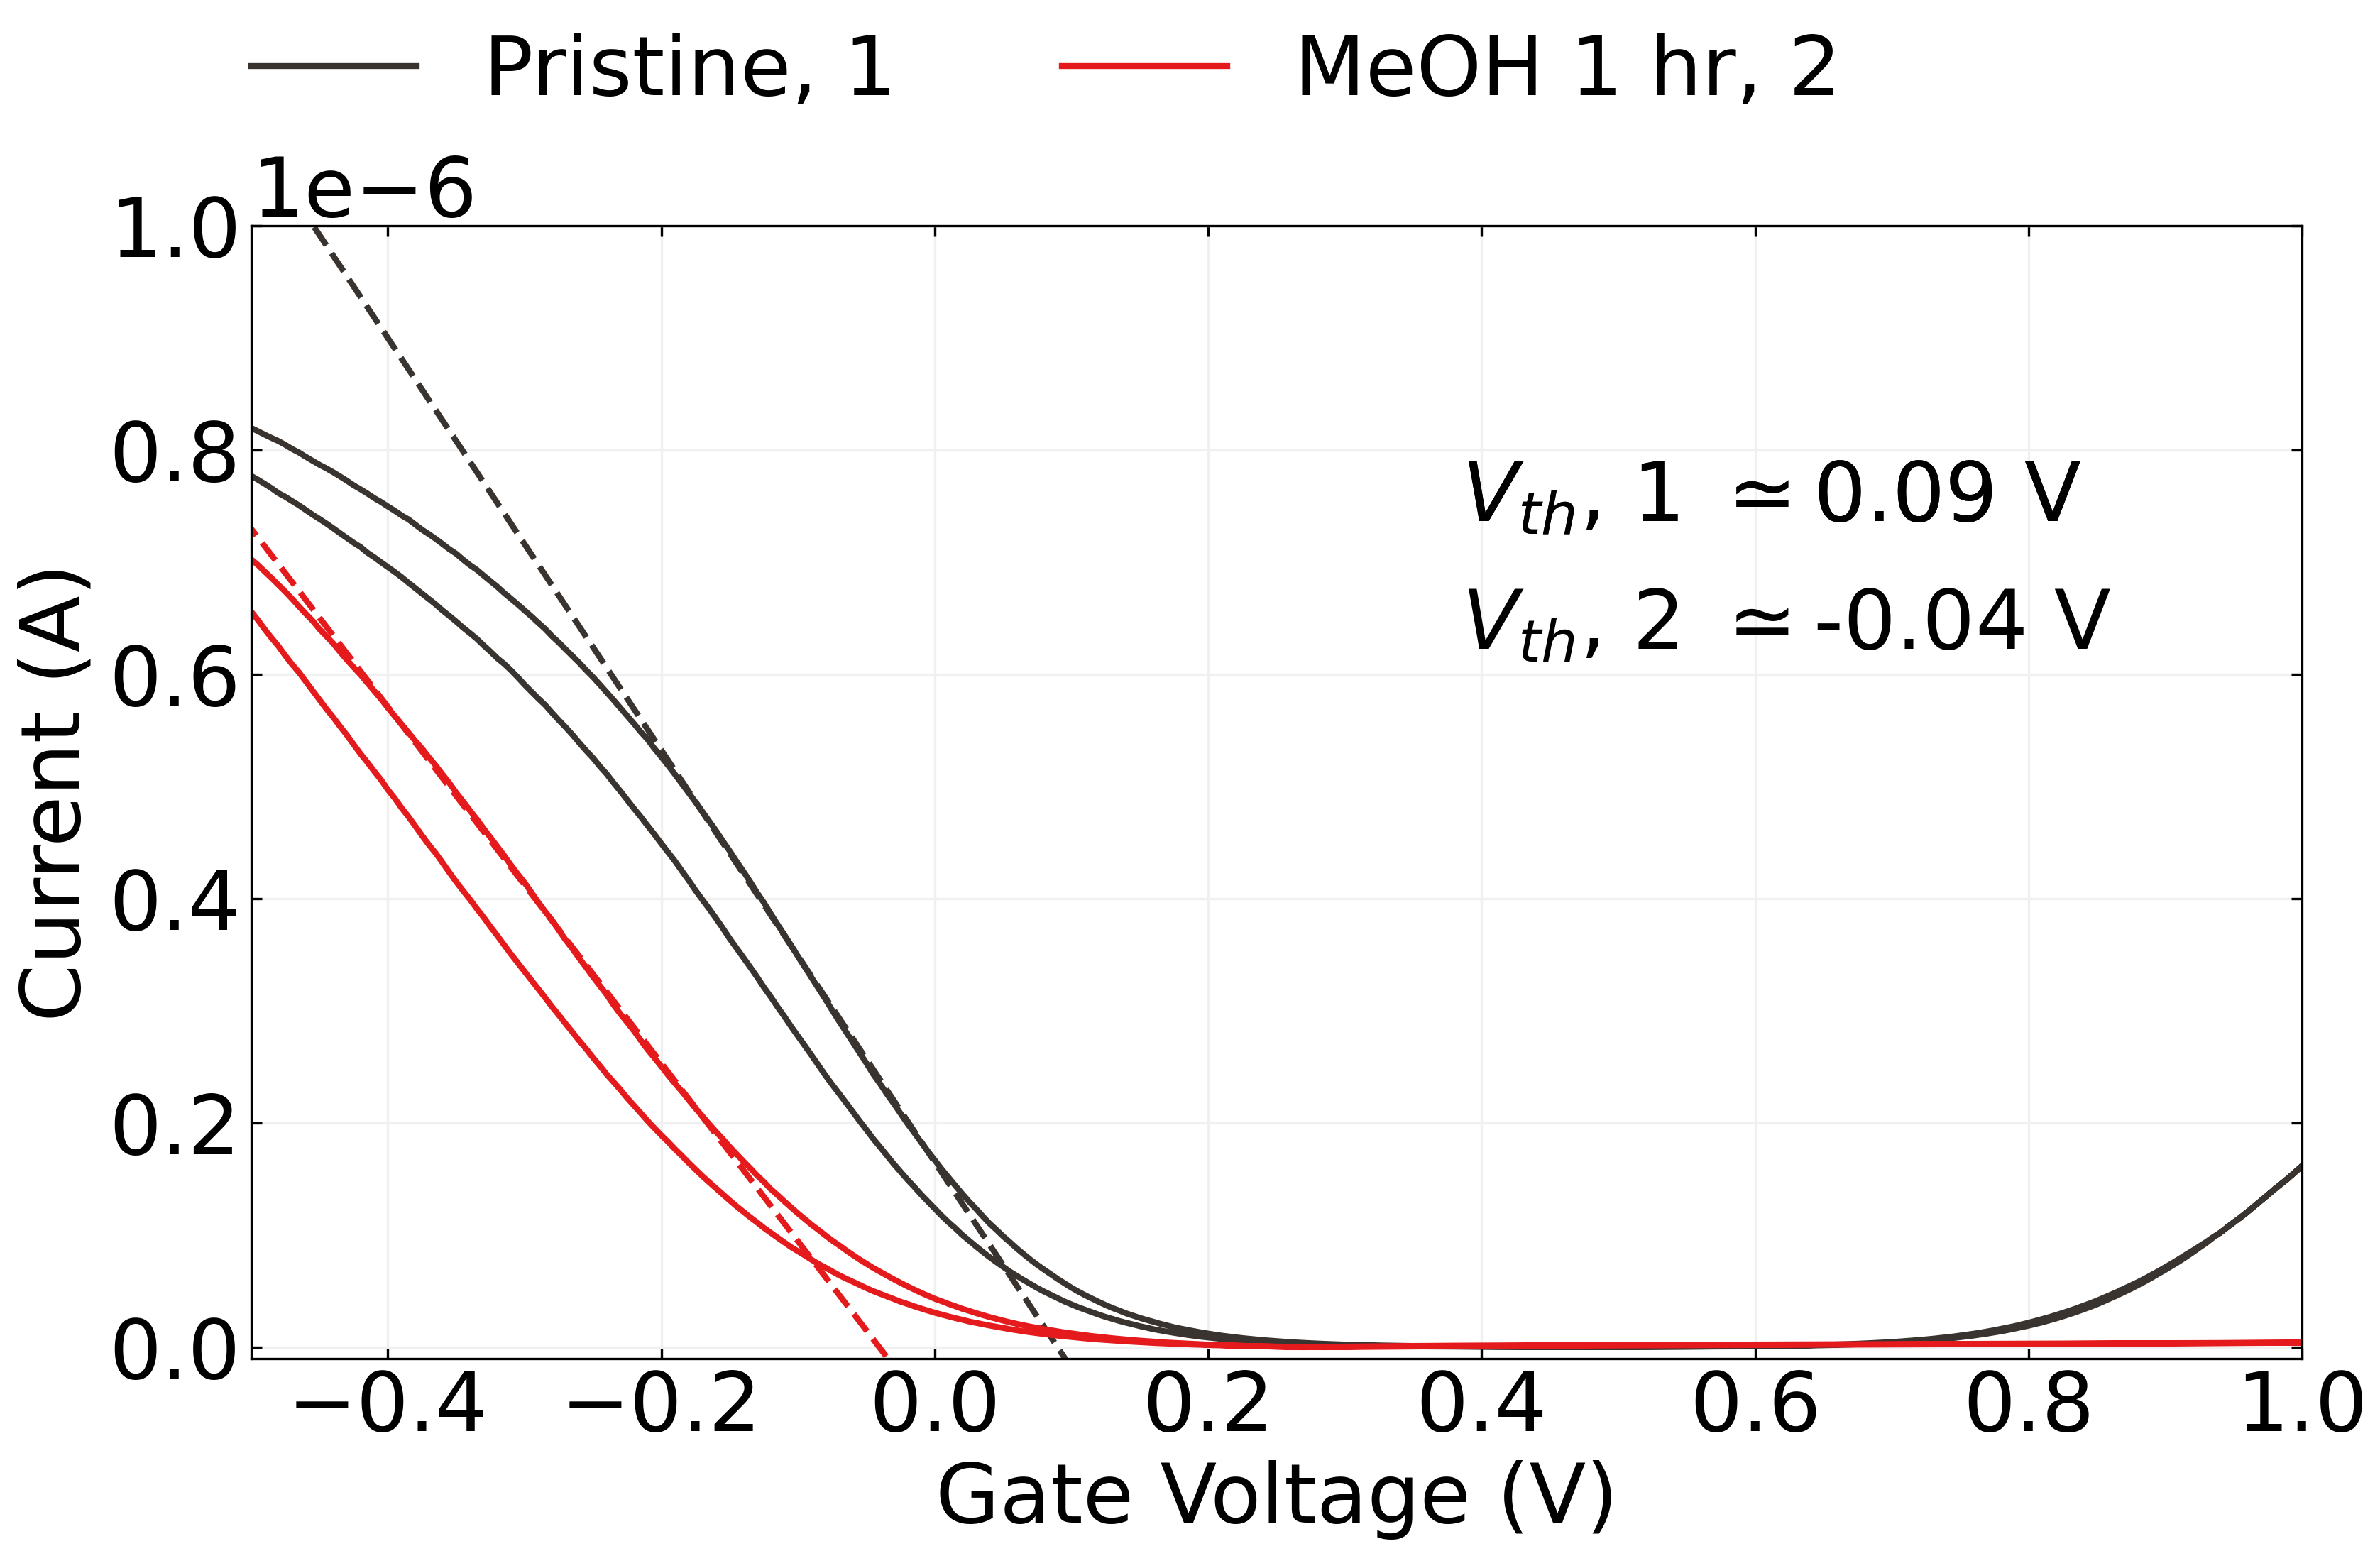
\includegraphics{./figures/ch6/Q23D5_ch1_MeOHonly.png}

}

}

\subcaption{\label{fig-meoh-only-tx}}
\end{minipage}%
%
\begin{minipage}[t]{0.50\linewidth}

{\centering 

\raisebox{-\height}{

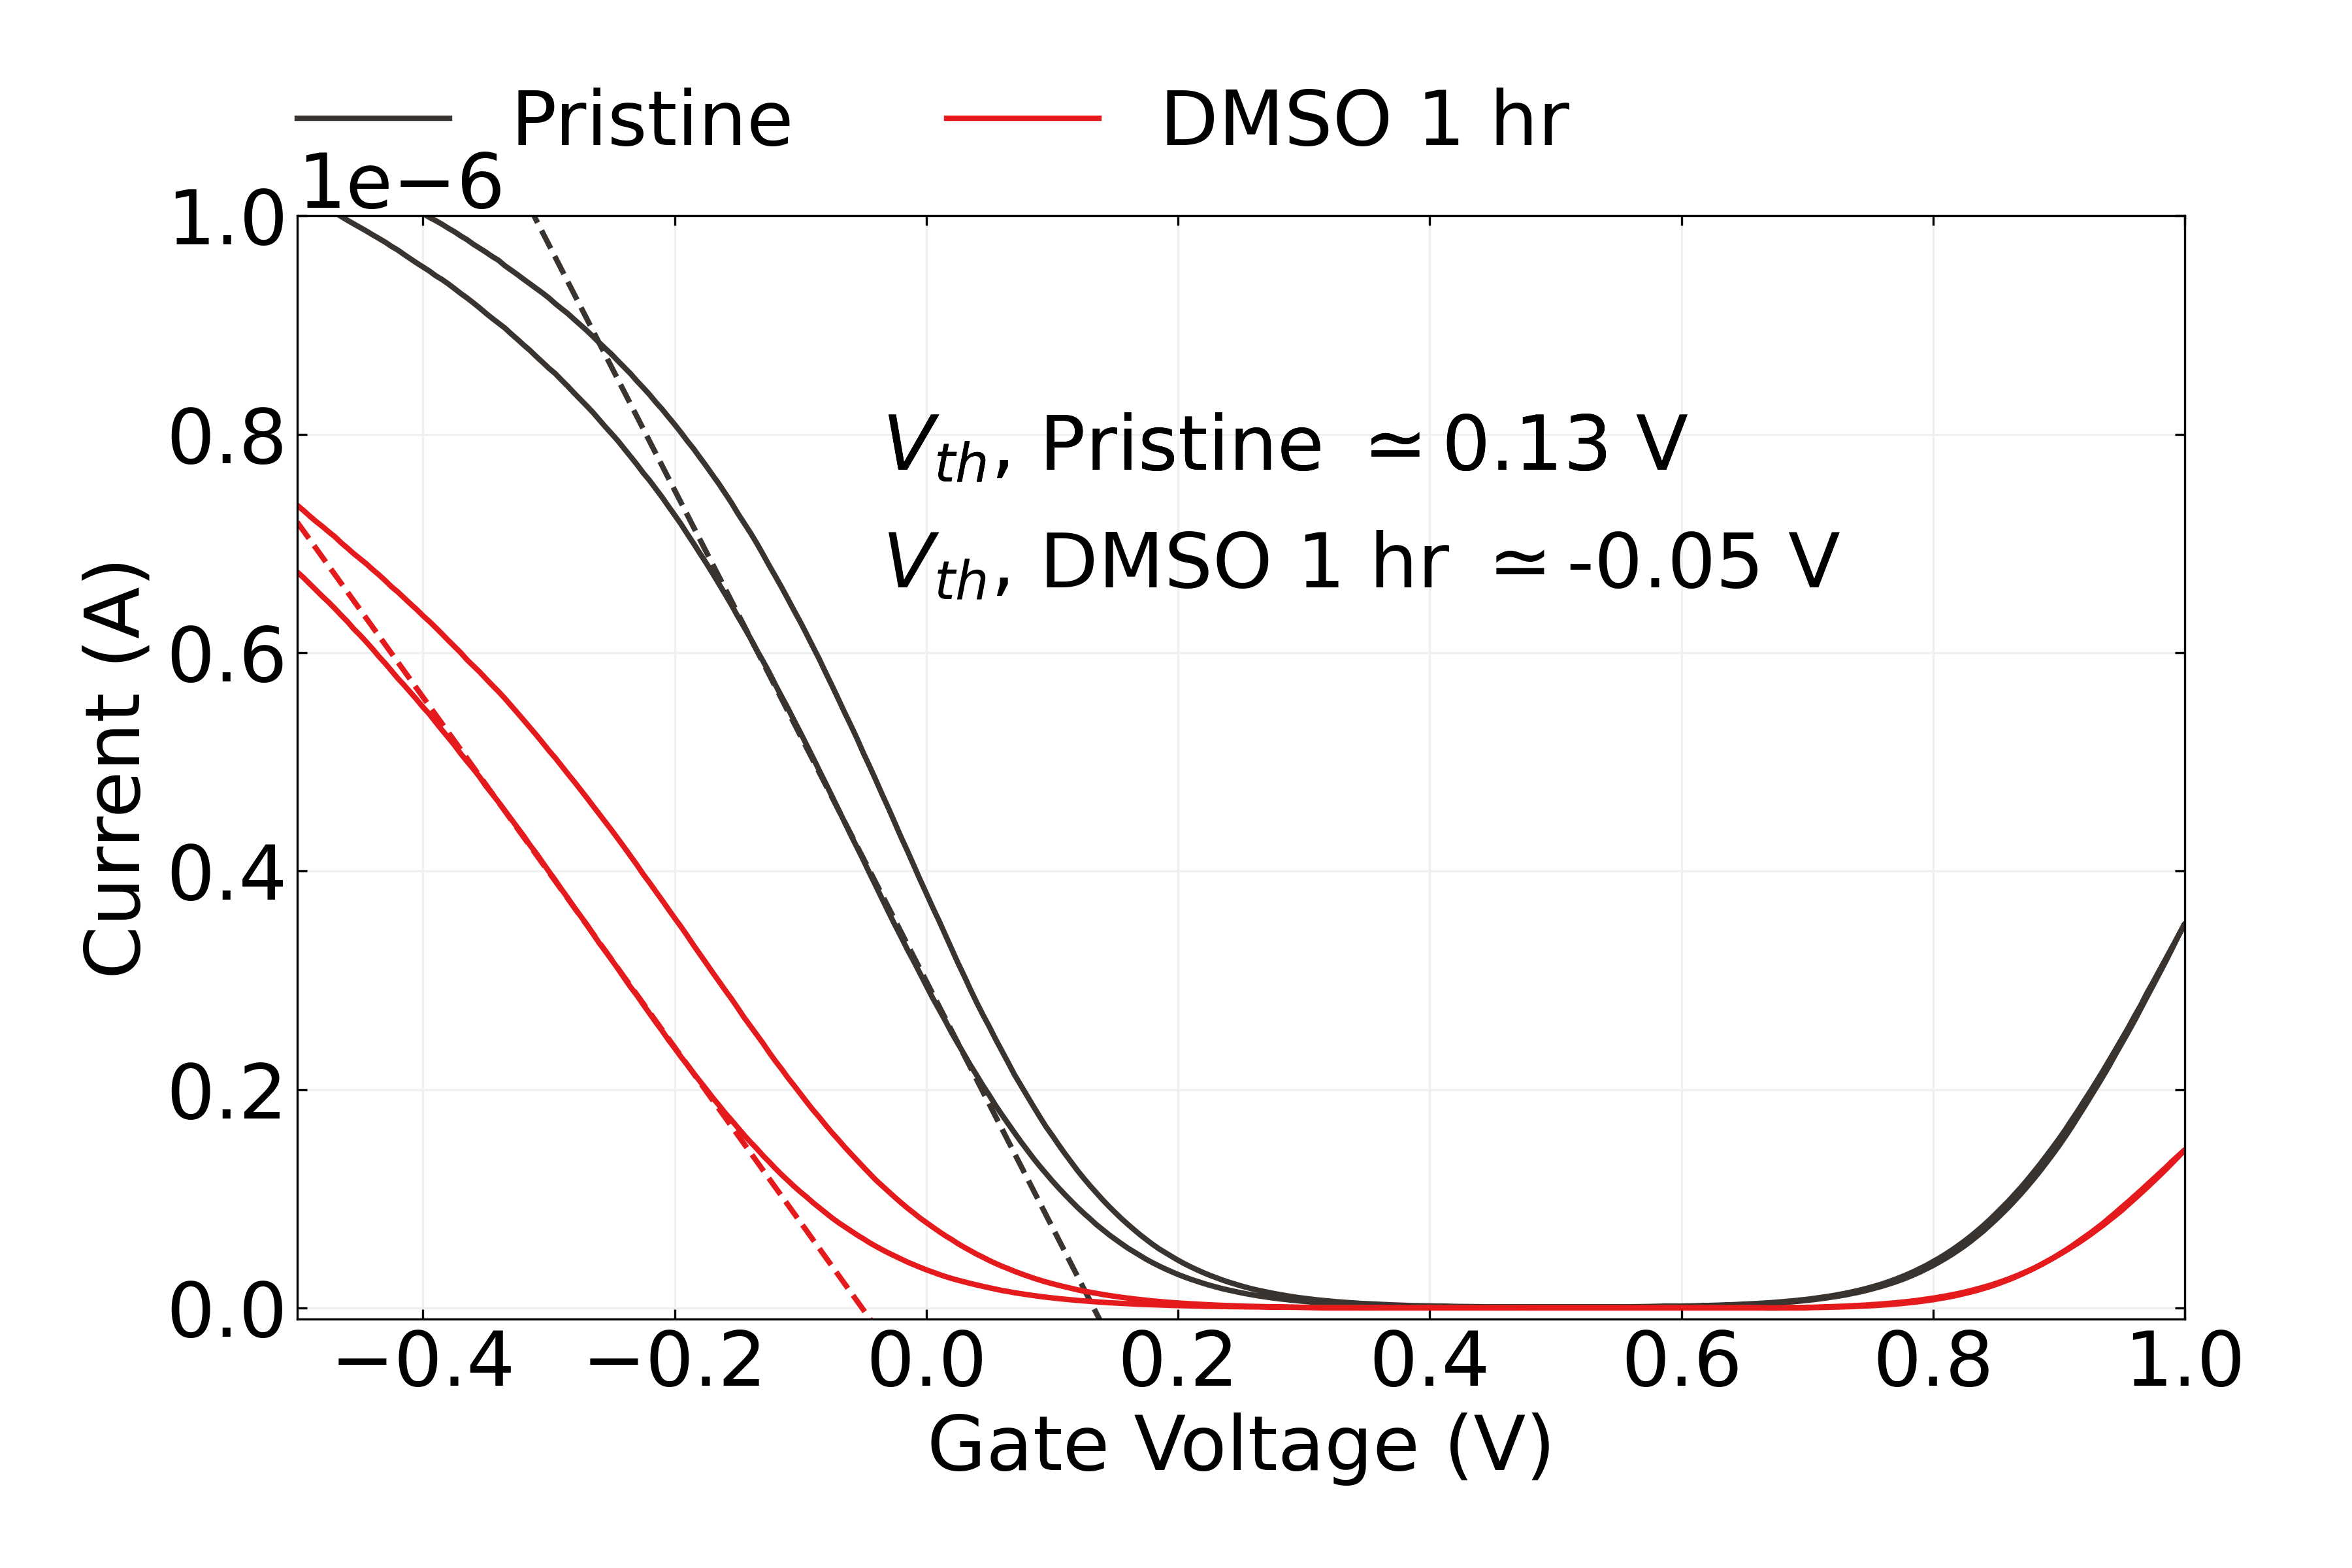
\includegraphics{./figures/ch6/Q23D12_ch1_DMSOonly.png}

}

}

\subcaption{\label{fig-dmso-only-tx}}
\end{minipage}%
\newline
\begin{minipage}[t]{0.50\linewidth}

{\centering 

\raisebox{-\height}{

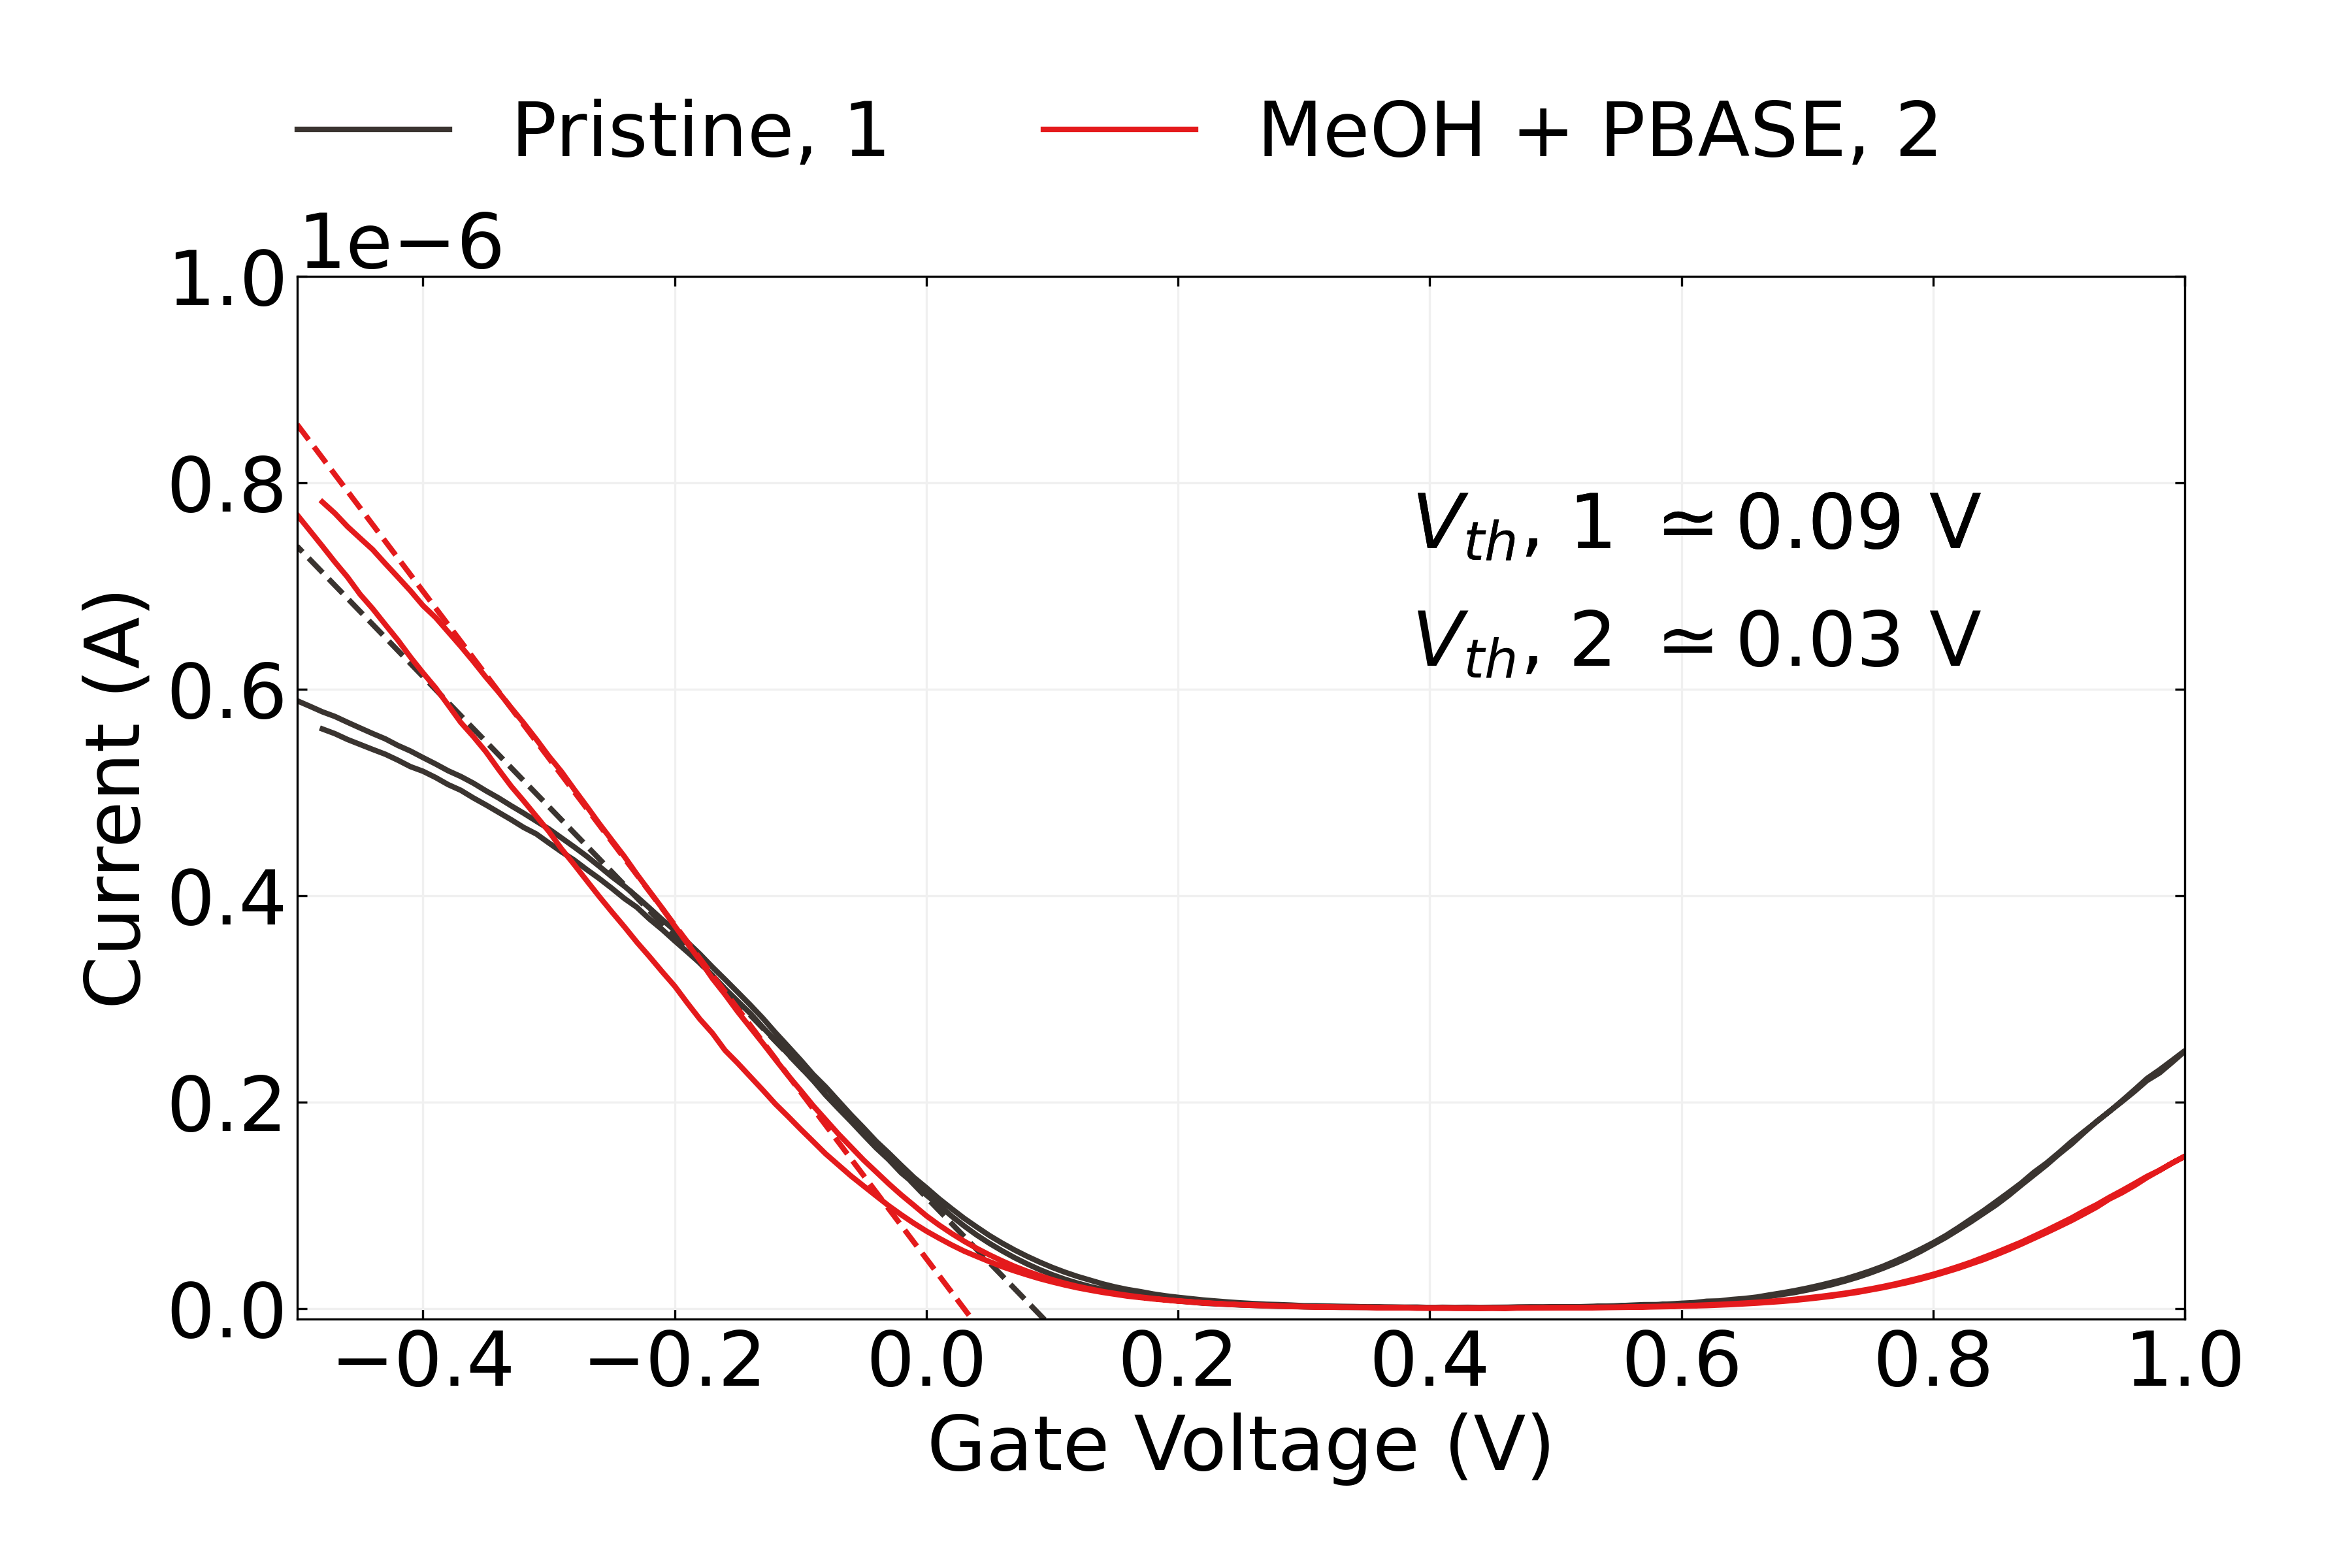
\includegraphics{./figures/ch6/Q2C6_ch2_MeOHPBASE.png}

}

}

\subcaption{\label{fig-meoh-pbase-tx}}
\end{minipage}%
%
\begin{minipage}[t]{0.50\linewidth}

{\centering 

\raisebox{-\height}{

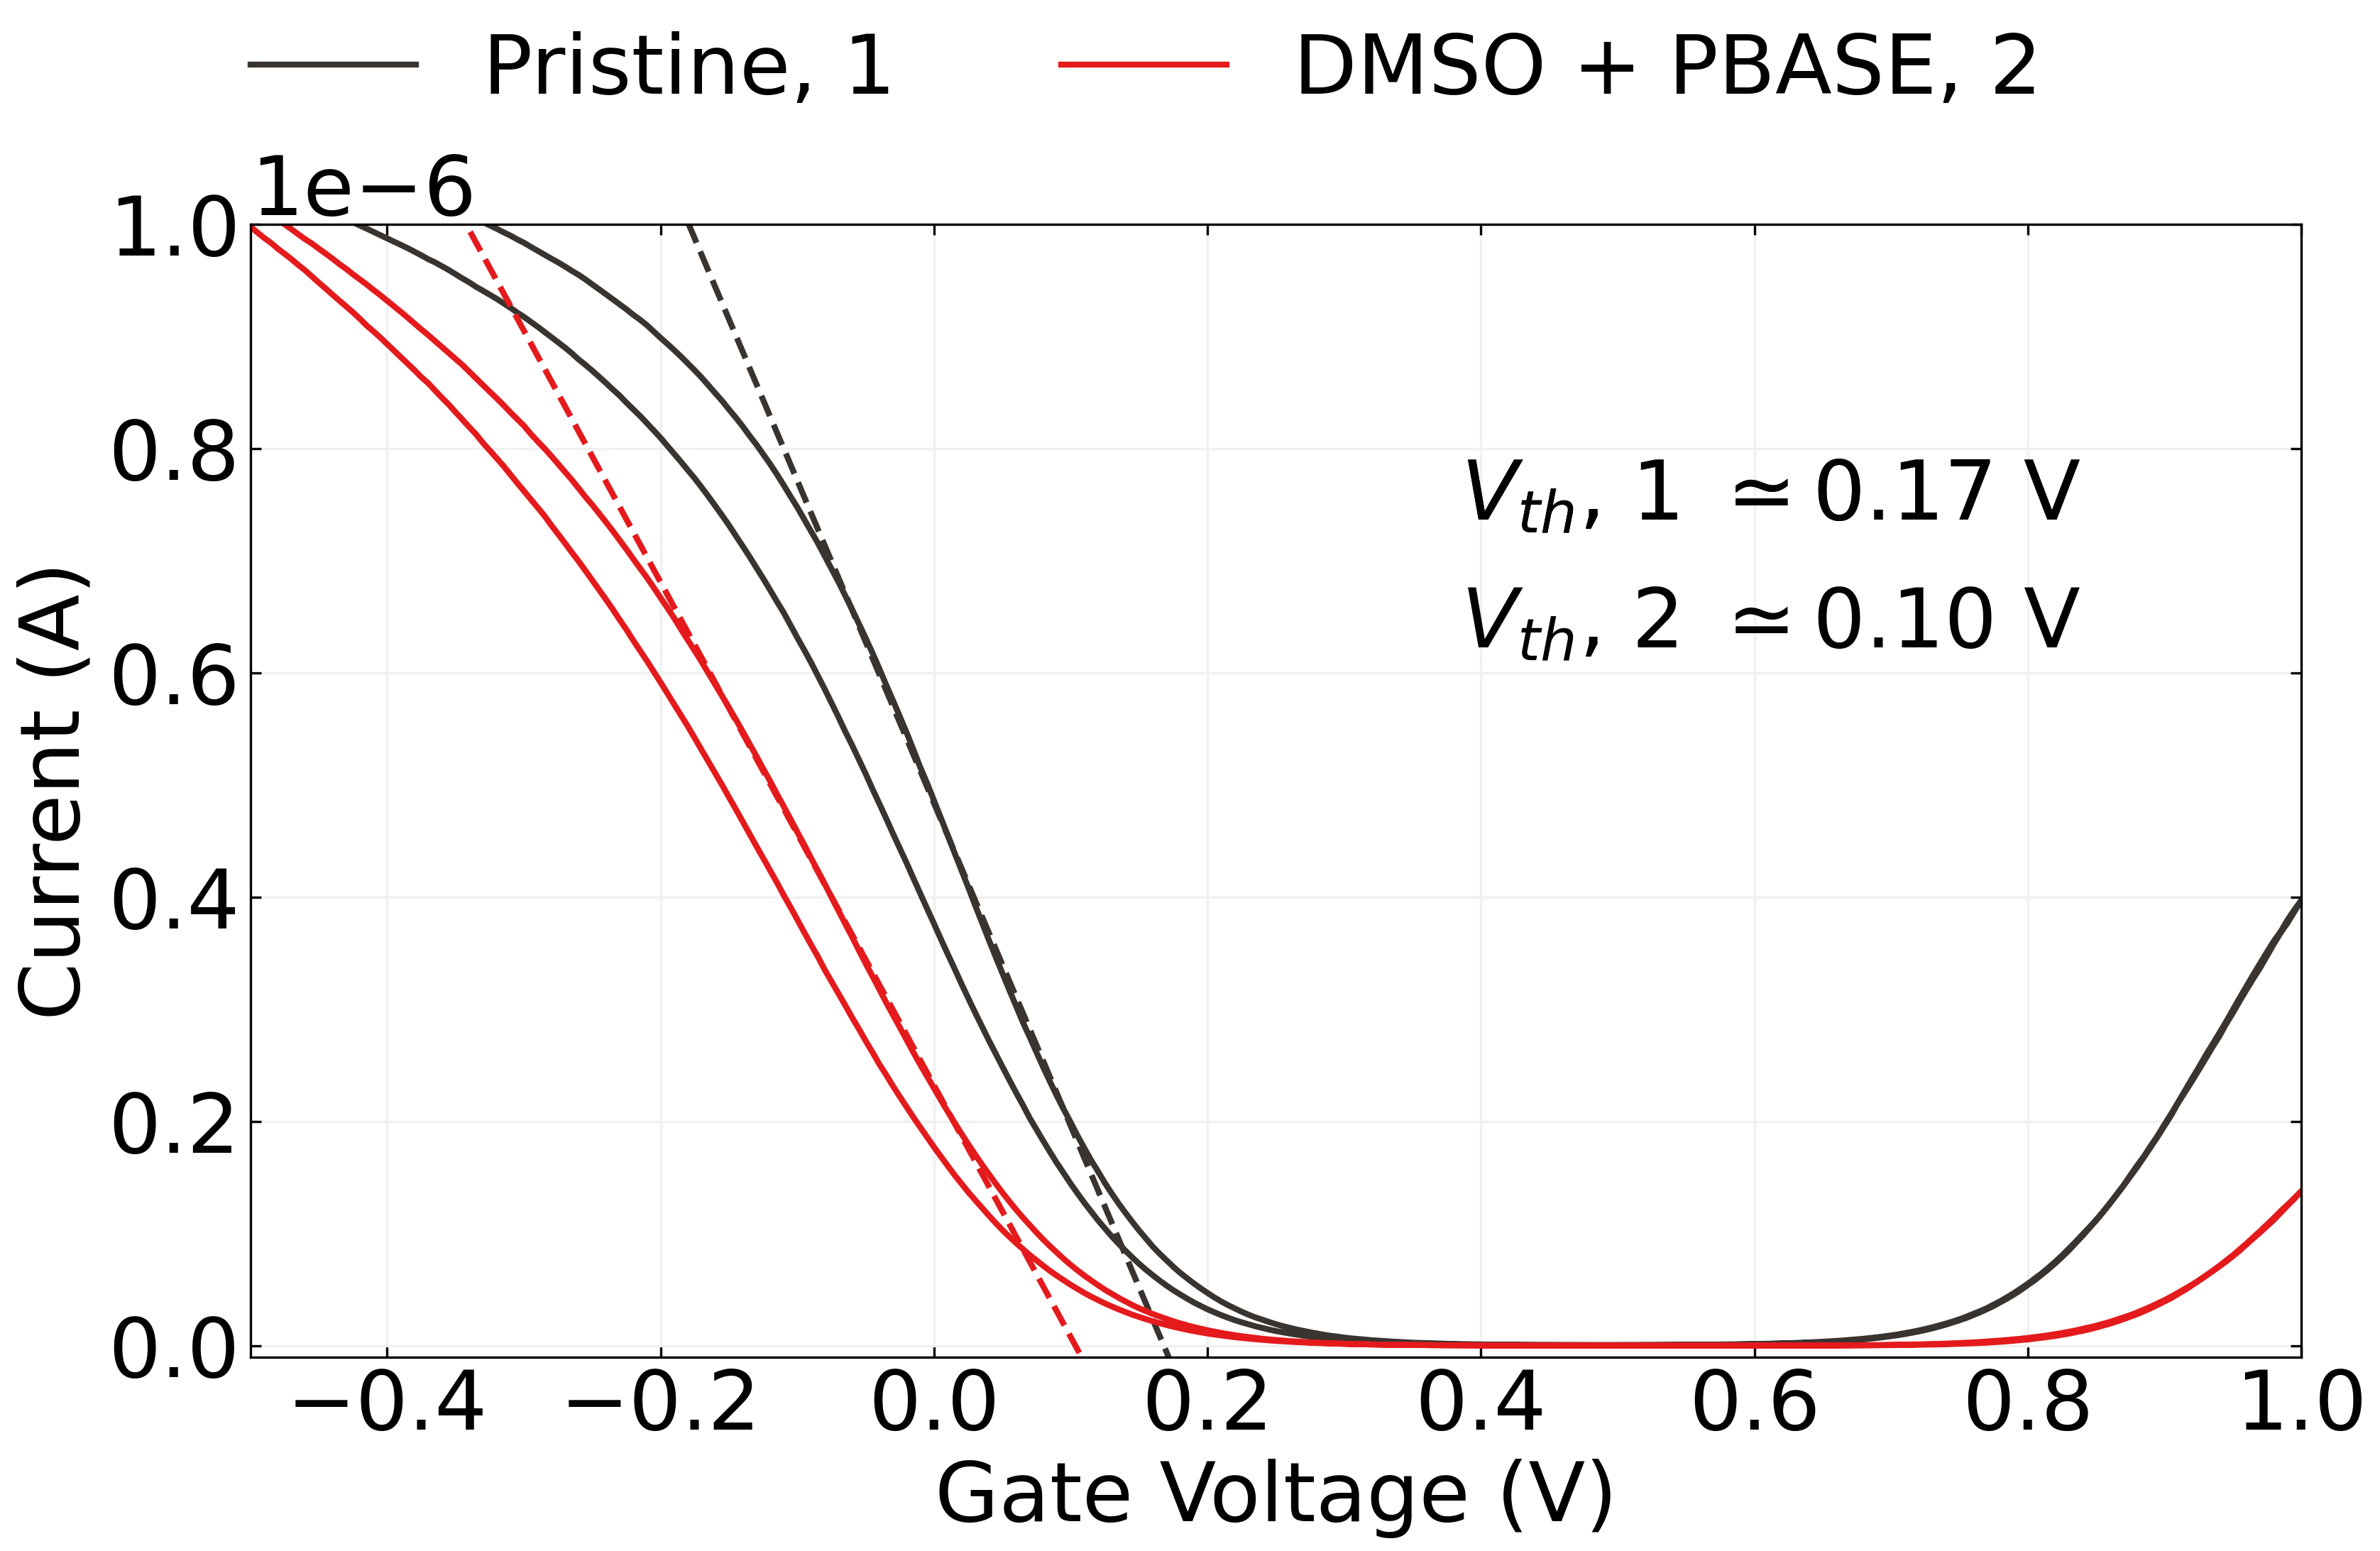
\includegraphics{./figures/ch6/Q23D7_ch3_DMSOPBASE.png}

}

}

\subcaption{\label{fig-dmso-pbase-tx}}
\end{minipage}%

\caption{\label{fig-PBASE-vs-solvent-only}The change in the electrical
transfer characteristics of carbon nanotube transistors after being
submerged in solvent for one hour and then rinsed thoroughly is
demonstrated in (a) and (b), where the solvents used are methanol (MeOH)
and dimethyl sulfoxide (DMSO) respectively. The change in
characteristics of similar transistor channels after being submerged in
these same solvents for one hour along with 1 mM PBASE then rinsed are
shown in (c) and (d) respectively. Threshold voltages for each transfer
characteristic are also shown.}

\end{figure}

The electrical characteristics of the carbon nanotube or graphene
transistor are often used to verify successful functionalisation and
make a statement about the effect of chemical modification on the
channel. However, this verification usually does not account for the
effect of the solvent on the transistor channel.
Figure~\ref{fig-meoh-only-tx} and Figure~\ref{fig-dmso-only-tx} show
that by exposing a carbon nanotube network channel to solvents commonly
used in PBASE functionalisation processes
(Table~\ref{tbl-pbase-functionalisation}), such as methanol (MeOH) or
dimethyl sulfoxide (DMSO), a significant negative shift in channel
threshold voltage occurs even after thorough rinsing with deionised
water. Besteman \emph{et al.} reported observing a similar effect from
prolonged exposure of a single carbon nanotube to dimethylformamide
(DMF) \autocite{Besteman2003}. It appears that the carbon nanotubes have
adsorped solvent which persists even after device cleaning. From the
shape of the change in the transfer curve, it seems the residual polar
solvent molecules capacitively gate the channel
\autocite{Artyukhin2006,Heller2008}.

In contrast, previous work has shown that \(\pi\)-stacking carbon
nanotube network to PBASE does not significantly affect the channel
gating and therefore the channel threshold voltage
\autocite{Besteman2003,Murugathas2019b}. Murugathas \emph{et al.}
observed a slight increase in channel conductance after PBASE
functionalisation. In Figure~\ref{fig-PBASE-vs-solvent-only}, we also
observe a slight increase in channel conductance post-functionalisation
for both Figure~\ref{fig-meoh-pbase-tx} and
Figure~\ref{fig-dmso-pbase-tx} relative to the solvent-only case in
Figure~\ref{fig-meoh-only-tx} and Figure~\ref{fig-dmso-only-tx}. It
appears that the presence of PBASE molecules increases channel mobility
and therefore conductance \autocite{Heller2008}.

Capactive gating results from dense coverage of adsorped molecules on
the carbon nanotube surface which have a low permittivity relative to
the surrounding electrolyte \autocite{Heller2008}. The relative
permittivity of MeOH and DMSO are \(\sim\) 33 \autocite{Mohsen-Nia2010}
and \(\sim\) 47 \autocite{Hunger2010} respectively, which are both much
lower than the relative permittivity of phosphate buffer saline,
\(\sim\) 80 \autocite{Salmanzadeh2013}. From
Figure~\ref{fig-meoh-only-tx} and Figure~\ref{fig-dmso-only-tx}, we find
the average threshold shift values resulting from exposure to each
solvent were \(\Delta\)V = \(-0.15 \pm 0.03\) V and \(\Delta\)V =
\(-0.15 \pm 0.01\) for MeOH and DMSO respectively. The threshold voltage
shifts in Figure~\ref{fig-meoh-pbase-tx} and
Figure~\ref{fig-dmso-pbase-tx} from the pristine are small compared with
the devices exposed to solvent only - this is likely due to the effect
of increased conductance from the PBASE competing with the gating effect
from the residual solvent.

This example illustrates why the use of electrical characteristics when
making conclusions around a successful functionalisation process should
individually take into account each substance used in the process. The
qualitative presence of a change in characteristics (or lack of one)
over the full process is not sufficient to make conclusive remarks about
the electrical changes due to functionalisation. A full set of
electrical control measurements are required for an understanding of
electronic changes occuring during the functionalisation process, in the
manner of Besteman \emph{et al.} \autocite{Besteman2003}.

\hypertarget{sec-other-linkers}{%
\subsection{Other Pyrene-Based Linkers}\label{sec-other-linkers}}

Alongside PBASE, there are a wide range of other pyrene-based linker
molecules used for modification of carbon nanotubes and graphene
\autocite{Zhou2019}. A few of these linkers are examined further below.

\hypertarget{pyrenebutyric-acid-pba-with-edcnhs}{%
\subsubsection*{1-Pyrenebutyric Acid (PBA) with
EDC/NHS}\label{pyrenebutyric-acid-pba-with-edcnhs}}
\addcontentsline{toc}{subsubsection}{1-Pyrenebutyric Acid (PBA) with
EDC/NHS}

Another linker molecule that can be used to attach receptor molecules to
a carbon nanotube or graphene channel is 1-pyrenebutyric acid (PBA). As
with PBASE, the pyrene group of PBA has a \(\pi\) interaction with the
carbon rings of the channel surface. It is possible to react PBA with
1-ethyl-3-(3-dimethylaminopropyl) carbodiimide hydrochloride (EDC or
EDAC) to form an \emph{O}-acylisourea intermediate, which can then react
with an amine group on a biomolecule and form an amide bond
\autocite{Sehgal1994,Hermanson2013-4}. The water solubility of EDC means
that, unlike PBASE, it is possible to functionalise with EDC dissolved
in water rather than in an organic solvent. However, like PBASE, EDC and
the \emph{O}-acylisourea intermediate are prone to hydrolysis,
especially in acidic conditions. Therefore, like PBASE, it should be
stored at −20\(^\circ\)C, and warmed to room temperature to prevent
condensation build-up, since exposure to condensation will hydrolyse the
reagent \autocite{Hermanson2013-4}. Furthermore, by adding
N-Hydroxysuccinimide (NHS) or N-hydroxysulfosuccinimide (sulfo-NHS) to
the reaction vessel, PBASE is formed as an active intermediate, which is
less prone to hydrolysis and increases the PBA/EDC reaction yield
\autocite{Sehgal1994,Hermanson2013-4,Hermanson2013-14}.

From Table~\ref{tbl-pbase-functionalisation} and
Table~\ref{tbl-pba-functionalisation}, we see that PBASE is more widely
used for non-covalent functionalisation than PBA/EDC. As was the case
for PBASE, there are a wide range of process variables used for the
functionalisation process, with little justification used for variables
chosen. Also notable is the frequent use of polyethylene glycol (PEG) or
pyrene-PEG for prevention of non-specific binding (see
\textbf{?@sec-non-specific-binding} for further discussion of NSB).
Despite being less widely useS, Mishyn \emph{et al.} state a preference
for the use of PBA/EDC over PBASE, as they found it was less prone to
hydrolysis and gave a larger reaction yield when binding ferrocene to
graphene \autocite{Mishyn2022}. A potential downside of using PBA/EDC
for protein immobilisation is that EDC has numerous ways of interacting
with proteins, and not all of these are necessarily desirable. The
addition of NHS may also cause processing issues, such as precipitation
of the reaction compound \autocite{Hermanson2013-4}. The greater range
of process variables involved in the functionalisation also adds to the
complexity of accurately reproducing past results.

\begin{figure}

{\centering 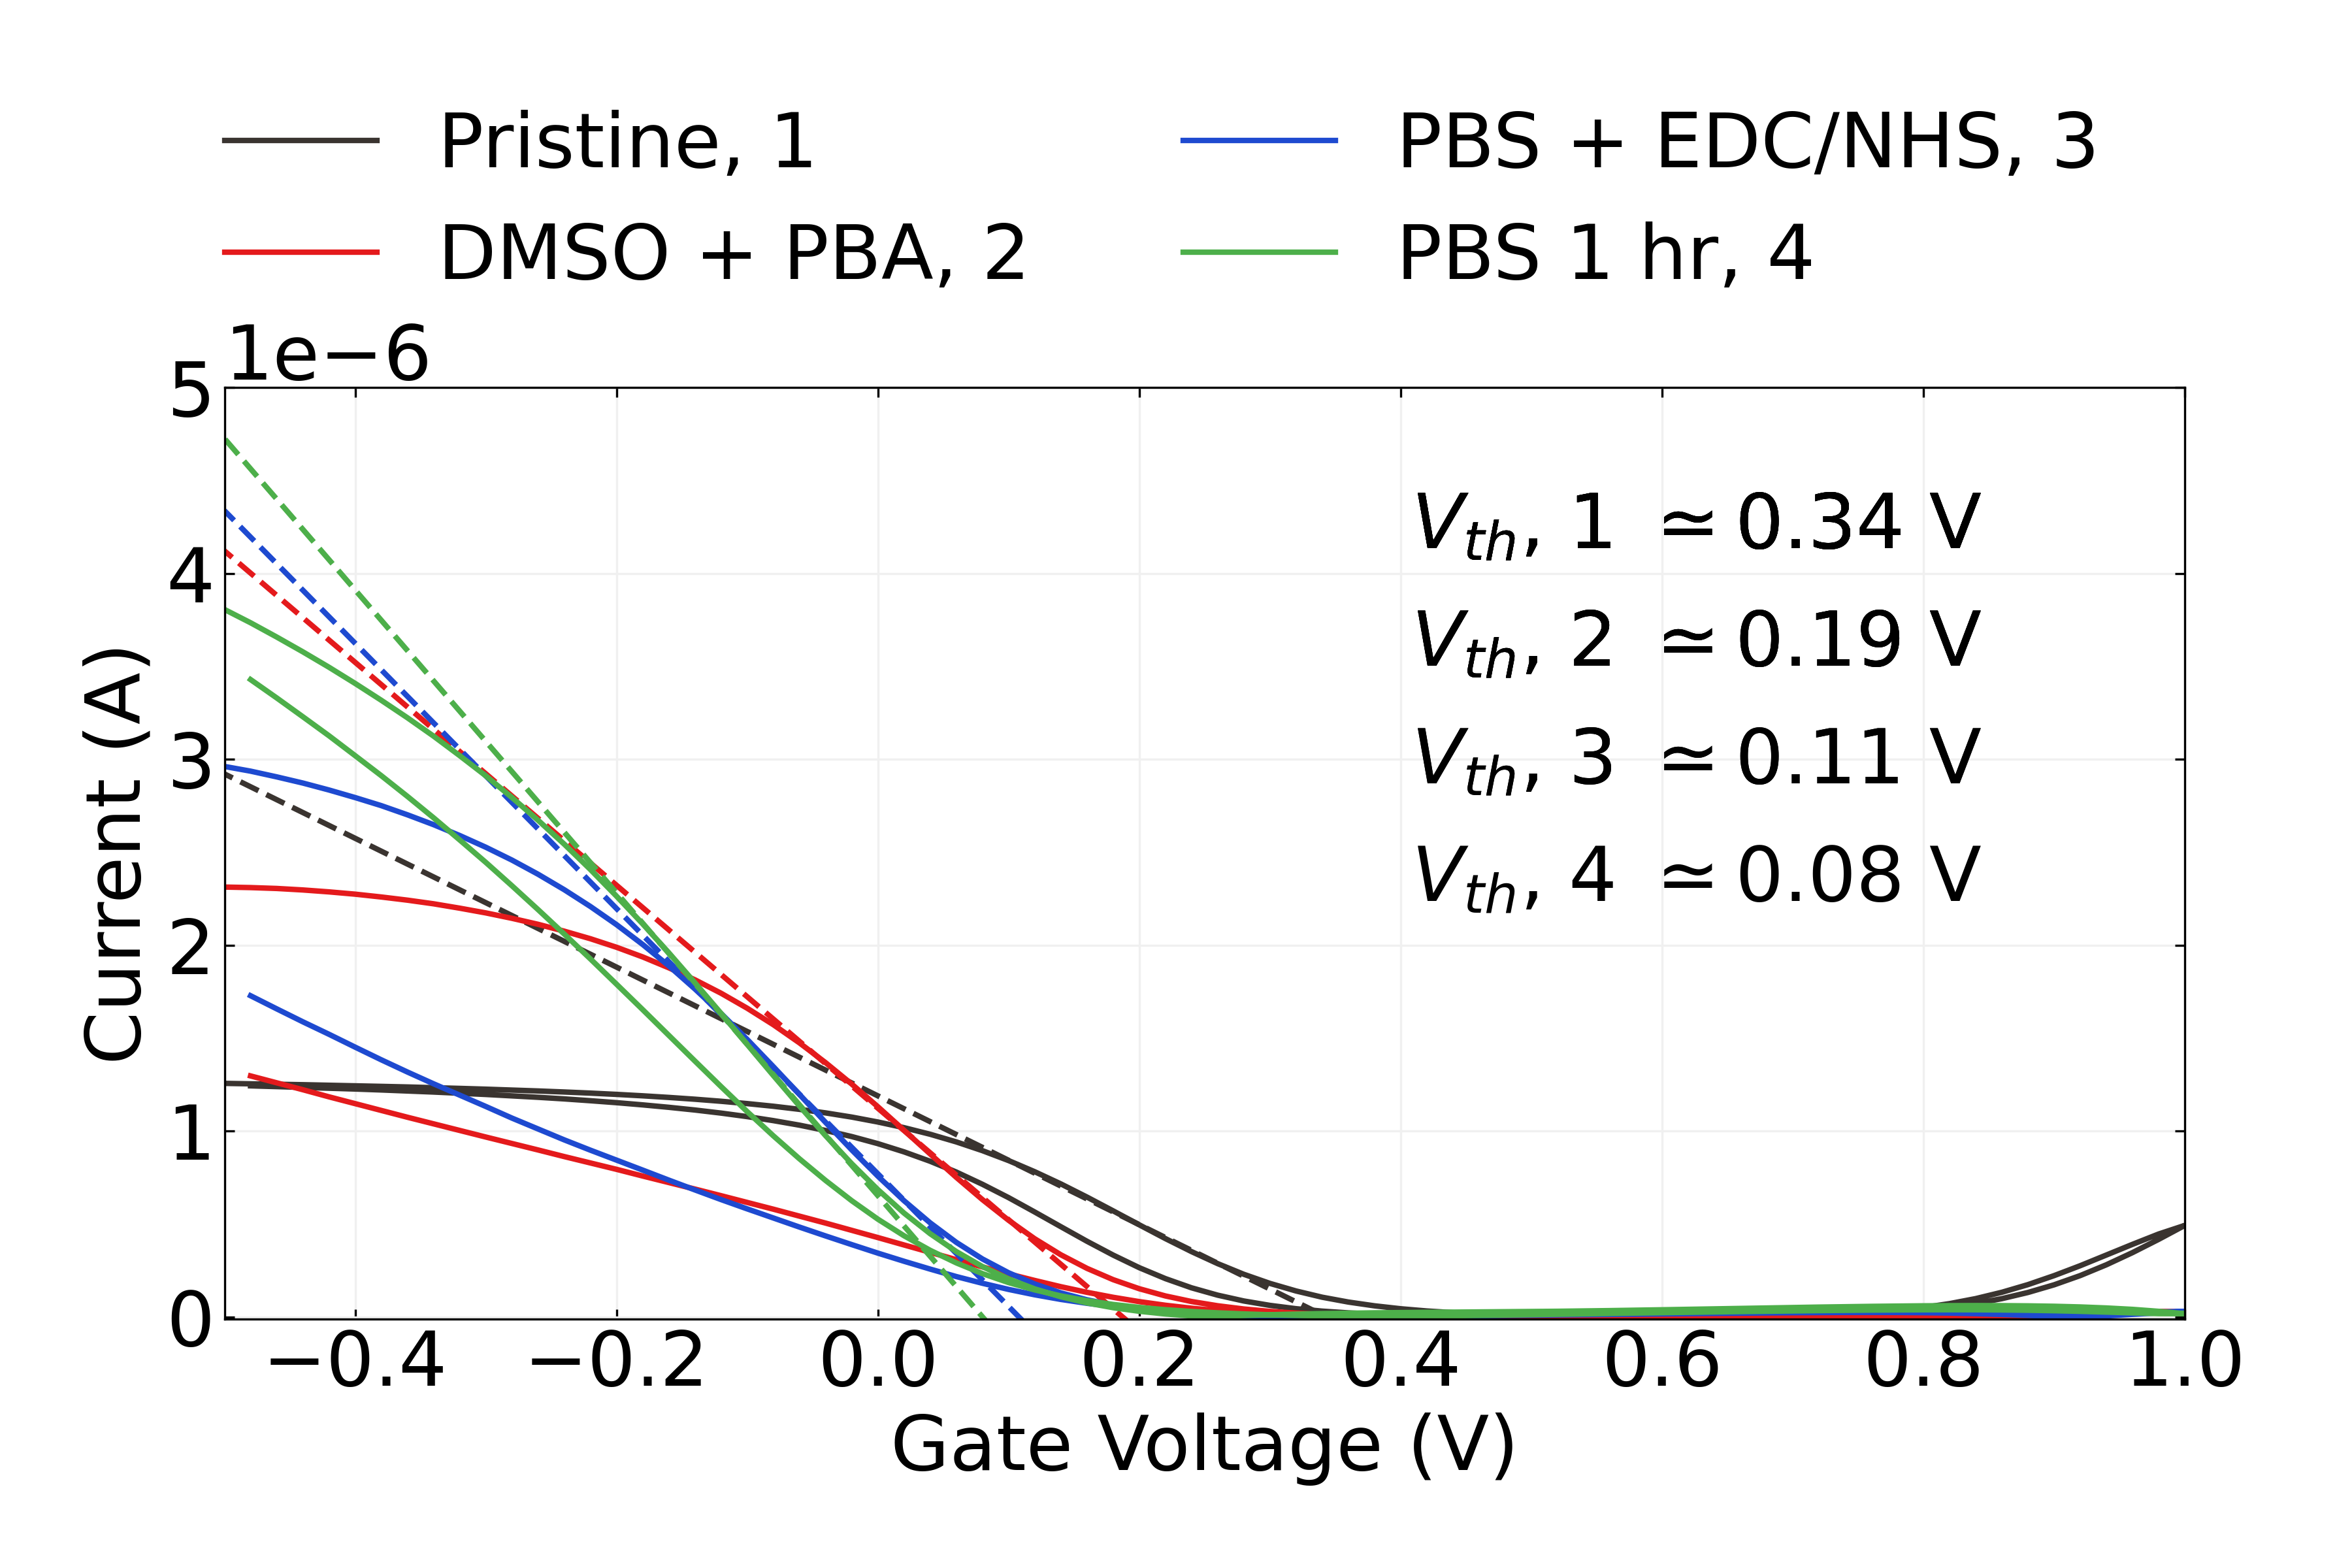
\includegraphics[width=0.7\textwidth,height=\textheight]{./figures/ch6/NTQ24C10_ch2_PBA.png}

}

\caption{\label{fig-pba-threshold-shift}Electrical transfer
characteristics of a carbon nanotube transistor before
functionalisation, after being submerged in DMSO containing 5 mM PBA for
1 hour, after being submerged in 1XPBS containing 20 mM EDC and 40 mM
NHS for 30 min, then after being submerged in fresh 1XPBS for 1 hour.
Threshold voltages for each transfer characteristic are also shown.}

\end{figure}

\newpage
\KOMAoptions{paper=landscape,pagesize}

\hfill\break
\hfill\break
\hfill\break

\hypertarget{tbl-pba-functionalisation}{}
\begin{longtable}[]{@{}llllllll@{}}
\caption{\label{tbl-pba-functionalisation}Comparison of 1-pyrenebutyric
acid (PBA) functionalisation processes used for immobilisation of
proteins and aptamers onto carbon nanotubes and graphene.
1-ethyl-3-(3-dimethylaminopropyl) carbodiimide hydrochloride (EDC) and
NHS were co-mingled in buffer/electrolyte solution or DI water in each
process - some papers used N-hydroxysulfosuccinimide instead of
N-hydroxysuccinimide, and both compounds are abbreviated to NHS in this
table. \(^†\)PEG or PEG pyrene were used to reduce non-specific binding.
\(^{††}\)Several pyrene-based linkers were compared and PBA was found to
give an optimal result.}\tabularnewline
\toprule()
Solvent & Channel & PBA (mM) & PBA Time (hr) & EDC (mM) & NHS (mM) &
EDC/NHS Time (hr) & References \\
\midrule()
\endfirsthead
\toprule()
Solvent & Channel & PBA (mM) & PBA Time (hr) & EDC (mM) & NHS (mM) &
EDC/NHS Time (hr) & References \\
\midrule()
\endhead
DMF & Graphene & 0.6 & 1 & - & - & 120 & Gao \textit{et al.}\(^†\)
\cite{Gao2016} \\
& & 5 & 2 & 2 & 5 & 30 & Mishyn \textit{et al.} \cite{Mishyn2022} \\
& CNT & 100 & 3 & 200 & - & 30 & Min \textit{et al.} \cite{Min2012} \\
DI water & CNT & - & - & 32 & 12 & Overnight & Pacios
\textit{et al.}\(^†\) \cite{Pacios2012} \\
Ethanol & CNT & 1 & 1 & 100 & 100 & 20 & Filipiak \textit{et al.}\(^†\)
\cite{Filipiak2018} \\
Acetonitrile & Graphene & 1 & 1 & 400 & 100 & 60 & Tong
\textit{et al.}\(^{††}\) \cite{Tong2020} \\
Borax solution & CNT & 2 & 24 & 2.5 & - & 1080 & Liu
\textit{et al.}\(^†\) \cite{Liu2011} \\
DMSO & Graphene & 5 & 1 & 50 & 50 & 90 & Fenzl \textit{et al.}
\cite{Fenzl2017} \\
\bottomrule()
\end{longtable}

\newpage
\KOMAoptions{paper=portrait,pagesize}

Figure~\ref{fig-pba-threshold-shift} shows the transfer characteristics
of a carbon nanotube transistor at various stages of a PBA/EDC
functionalisation, where a excess of N-hydroxysuccinimide (NHS) was
added alongside EDC. The PBA was dissolved in DMSO, and the device
channels were exposed to this solution for 1 hour. Subsequently, it was
rinsed with 1XPBS and exposed to 20 mM EDC and 40 mM NHS in 1XPBS
electrolyte for 30 minutes. We can compare
Figure~\ref{fig-pba-threshold-shift} to
Figure~\ref{fig-PBASE-vs-solvent-only} for a better understanding of the
result of both the PBASE and PBA/EDC functionalisation methods. The
threshold shift with the addition of 5 mM PBA in DMSO for 1 hour is
equivalent to the shift seen when only DMSO is added, \(\Delta\)V =
-0.15 V. The lack of a significant threshold shift is a result of pyrene
having a neutral charge state, and any contributions from the charged
carboxyl group being screened from the carbon nanotube sidewalls by
surrounding water molecules \autocite{Lerner2012}. However, as in the
case of the addition of PBASE, there also appears to be an increase in
hole mobility, which may be due to the pyrene groups increasing
connectivity within the carbon nanotube network
\autocite{Murugathas2019b}. When EDC/NHS is added, a further increase in
mobility of channel holes is seen \autocite{Heller2008}.

\hypertarget{pyrene-nta-pyrene-biotin-and-pegylation}{%
\subsubsection*{Pyrene-NTA, Pyrene-Biotin and
PEGylation}\label{pyrene-nta-pyrene-biotin-and-pegylation}}
\addcontentsline{toc}{subsubsection}{Pyrene-NTA, Pyrene-Biotin and
PEGylation}

Through chemical coupling/conjugation, it is possible to replace the NHS
ester group on PBASE with other groups that can undergo binding
reactions with proteins. For example, PBASE can be modified with
N\(\alpha\),N\(\alpha\)-Bis(carboxymethyl)-L-lysine hydrate (also known
as N-(5-Amino-1-carboxypentyl)iminodiacetic acid, AB-NTA) to produce
pyrene-nitrilotriacetic acid (pyrene-NTA). The attached NTA group is
able to chelate with metal ions such as Cu\(^{2+}\) or Ni\(^{2+}\),
which then can then coordinate with polyhistidine-tags attached to a
protein \autocite{Holzinger2011,Amano2016}. This functionalisation
procedure was successfully used with mammalian odorant receptors
attached via Ni\(^{2+}\) to a single carbon nanotube to detect eugenol
vapour in real-time \autocite{Goldsmith2011}. Pyrene-biotin (pyrene
butanol biotin ester) can also be produced for attaching avidin or
strepavidin \autocite{Holzinger2011}. As avidin and strepavidin are
tetrameric, they can be attached to both pyrene-biotin and biotinylated
proteins simultaneously via strong non-covalent bonding
\autocite{Star2003a,Dundas2013,Hermanson2013-11,Fairhead2015}. The use
of protein his-tags and avi-tags for these binding processes means
protein-transducer attachment can be better controlled than the amide
bonding discussed earlier, with high specificity and directionality.

It is also possible to attach polyethylene glycol (PEG) chains to a
pyrene group and modify them with reactive groups such as NTA and biotin
to attach proteins in the same manner outlined in the previous paragraph
\autocite{Hermanson2013-18,Meran2018}. Once modified with PEG, pyrene
linkers are also more water soluble, making it possible to perform a
full functionalisation procedure exclusively in aqueous solution
\autocite{Hermanson2013-18}. By setting the length of the PEG chain, the
size of the linker molecule can be controlled - selection of a short
chain is important for ensuring attached receptors remain within the
Debye length of the transducer \autocite{Shkodra2021}.

\hypertarget{verifying-pyrene-attachment-to-cnt-network-and-graphene}{%
\section{Verifying Pyrene Attachment to CNT network and
Graphene}\label{verifying-pyrene-attachment-to-cnt-network-and-graphene}}

\hypertarget{sec-photoresist-contamination}{%
\subsection{Photoresist
contamination}\label{sec-photoresist-contamination}}

\hypertarget{raman-spectroscopy}{%
\subsection{Raman Spectroscopy}\label{raman-spectroscopy}}

\hypertarget{pyrene-peg-fitc-fluorescence-microscopy}{%
\subsection{Pyrene-PEG-FITC fluorescence
microscopy}\label{pyrene-peg-fitc-fluorescence-microscopy}}

\hypertarget{plasma-clean-comparison}{%
\subsubsection*{Plasma clean comparison}\label{plasma-clean-comparison}}
\addcontentsline{toc}{subsubsection}{Plasma clean comparison}

\hypertarget{surfactant-comparison}{%
\subsubsection*{Surfactant comparison}\label{surfactant-comparison}}
\addcontentsline{toc}{subsubsection}{Surfactant comparison}

\hypertarget{pyrene-peg-electrical-characterisation}{%
\subsection{Pyrene-PEG electrical
characterisation}\label{pyrene-peg-electrical-characterisation}}

\appendix
\addcontentsline{toc}{part}{Appendices}

\hypertarget{sec-python}{%
\chapter{Python Code for Data Analysis}\label{sec-python}}

\hypertarget{code-repository}{%
\section{Code Repository}\label{code-repository}}

The code used for general analysis of field-effect transistor devices in
this thesis was written with Python 3.8.8. Contributors to the code used
include Erica Cassie, Erica Happe, Marissa Dierkes and Leo Browning. The
code is located on GitHub and the research group OneDrive, and is
available on request.

\hypertarget{sec-histogram-analysis}{%
\section{Atomic Force Microscope Histogram
Analysis}\label{sec-histogram-analysis}}

The purpose of this code is to analyse atomic force microscope (AFM)
images of carbon nanotube networks in .xyz format taken using an atomic
force microscope and processed in Gwyddion (see
\textbf{?@sec-afm-characterisation}). It was originally designed by
Erica Happe in Matlab, and adapted by Marissa Dierkes and myself for use
in Python.

\begin{equation}\protect\hypertarget{eq-lin-combo-gaussian}{}{
f(x) = k_1\exp{\Bigg(-\frac{{(x-m_1)}^{2}}{{2s_1}^{2}}\Bigg)} + k_2\exp{\Bigg(-\frac{{(x-m_2)}^{2}}{{2s_2}^{2}}\Bigg)} + ...
}\label{eq-lin-combo-gaussian}\end{equation}

The .xyz data is initially sorted into bins with 0.15 nm size. The bin
with the maximum number of counts is set at 0 nm, as this peak
represents the mean of the surface roughness of the bare silicon. The
parameters \(m_i\), \(s_i\), \(k_i\) (i = 1, 2, 3) are used with
objective function Equation~\ref{eq-lin-combo-gaussian} to overlay the
data with normal distributions. These fitting parameters represent the
mean (m), standard deviation (s) and amplitude (k) of each normal
distribution. We can make approximations of some of these fitting
parameters using the histogram data.

\(k_1\) is taken to be the maximum y-value of the data being fitted,
\(m_1\) is set to zero (used as a point of reference) and \(s_1\) is
taken as one-third of the difference between \(m_1\) and the x-value of
the first datapoint where the y-value is greater than 1\% of \(k_1\)
(approximating one standard deviation). We find the distribution given
by these values using Equation~\ref{eq-lin-combo-gaussian}, and subtract
it from the existing dataset.

Then, using the analysis technique outlined by Vobornik \emph{et al.}
\autocite{Vobornik2023} in Gwyddion, we manually find estimates for the
mean \(m_2\) and standard deviation \(s_2\) of the carbon nanotube
bundle distribution. We then take \(k_2\) to be the maximum y-value of
this modified dataset, and \(m_1\) to be the x-value of the maximum
y-value. We then set \(k_2\) so that the height of the resulting
distribution at one standard deviation matches the height of the .xyz
data histogram. We take this distribution, and subtract it from the
existing dataset.

The code also allows for discretely binning continuous data from fitted
normal distributions and examining the proportion of counts above or
below a particular height. 2.9 nm is roughly where 2 bundles with
average size 1.45 nm can start to be present, and is used as an estimate
of the boundary value between single-tube bundle diameters and
multi-tube bundle diameters.

\hypertarget{sec-field-effect-transistor-analysis}{%
\section{Field-Effect Transistor
Analysis}\label{sec-field-effect-transistor-analysis}}

The purpose of this code is to analyse electrical measurements taken of
field-effect transistor (FET) devices. Electrical measurements were
either taken from the Keysight 4156C Semiconductor Parameter Analyser,
National Instruments NI-PXIe or Keysight B1500A Semiconductor Device
Analyser as discussed in \textbf{?@sec-electrical-characterisation}; the
code is able to analyse data taken from all three measurement setups.
The main Python file in the code base consists of three related but
independent modules: the first analyses and plots sensing data from the
FET devices, the second analyses and plots transfer characteristics from
channels across a device, and the third compares individual channel
characteristics before and after a modification or after each of several
modifications. The code base also features a separate config file and
style sheet which govern the behaviour of the main code. The code base
was designed collaboratively by myself and Erica Cassie over GitHub
using the Sourcetree Git GUI.

The first of the three modules is for processing sensing datasets. This
module imports sensing measurements in .csv format and analyses them,
then outputs a plot of the raw data, alongside multiple plots which have
been modified in various ways. It can also fit exponential and linear
trendlines to regions of the sensing data, as well as find the signal
change per analyte addition, and returns spreadsheets containing the
results of these analyses. These spreadsheets include the standard
deviation for all included parameters. Modified plots include normalised
plots (type of normalisation can be set in config file), plots with
fitted curves, plots with the linear baseline drift removed, plots of
signal with analyte addition, ``despiked'' plots and ``filtered'' plots.
It is possible to add annotations to any of these plots using the config
file, and it is possible to produce a plot with a combination of these
modifications.

The scipy.optimize.curve\_fit module is used to fit linear and
exponential curves to regions of interest of the sensing data. Initial
parameters for the scipy.optimize.curve\_fit module are chosen by
approximating fitting parameters in a similar manner to the approach in
Section~\ref{sec-histogram-analysis}. For a linear fit \(mt + b\), the
parameters are simply set as \(m=1\) and \(b=0\). For an exponential fit
\(a\exp{(-t/\tau)} + c\), \(c\) is set as the final current measurement
of the region of interest and \(a\) is set as the initial current
measurement minus \(c\). Then, \(\tau\) is set as the time where current
has dropped to \(e^{-1}a + c\).

``Despiked'' plots have had spurious datapoints removed through the use
of an interquartile range rolling filter. The window size of the rolling
filter used was 40 datapoints, and datapoints in each window with a
z-score above \(\pm 3\) were removed from the plotted/processed data.
``Filtered'' plots had noise reduced using a moving median filter. The
moving median filter is more effective at removing noise than a simple
moving average, and has advantages over other filters (such as the
Savitzky-Golay filter) when removing noise from data with sharp edges,
as is the case for sensing data. Median filtering can also be used for
baseline drift compensation, though this approach was not used in this
thesis \autocite{Stone2011}. The moving median filter used had a window
of 40 datapoints.

Plots of signal with analyte addition were constructed from current data
after first removing baseline drift and applying a moving median filter.
A simple difference calculation between the mean of the filtered current
before an addition and the mean of the filtered current after the
addition was performed at each addition. These differences were then
normalised relative to the initial current. The signal with analyte
addition give reasonably consistent results regardless of whether
baseline drift was removed from the data, as shown in
Figure~\ref{fig-spaa-plot-comparison}. We can therefore be confident
that robust signal with analyte addition plots are robust even in the
presence of significant drift.

\begin{figure}

\begin{minipage}[t]{0.50\linewidth}

{\centering 

\raisebox{-\height}{

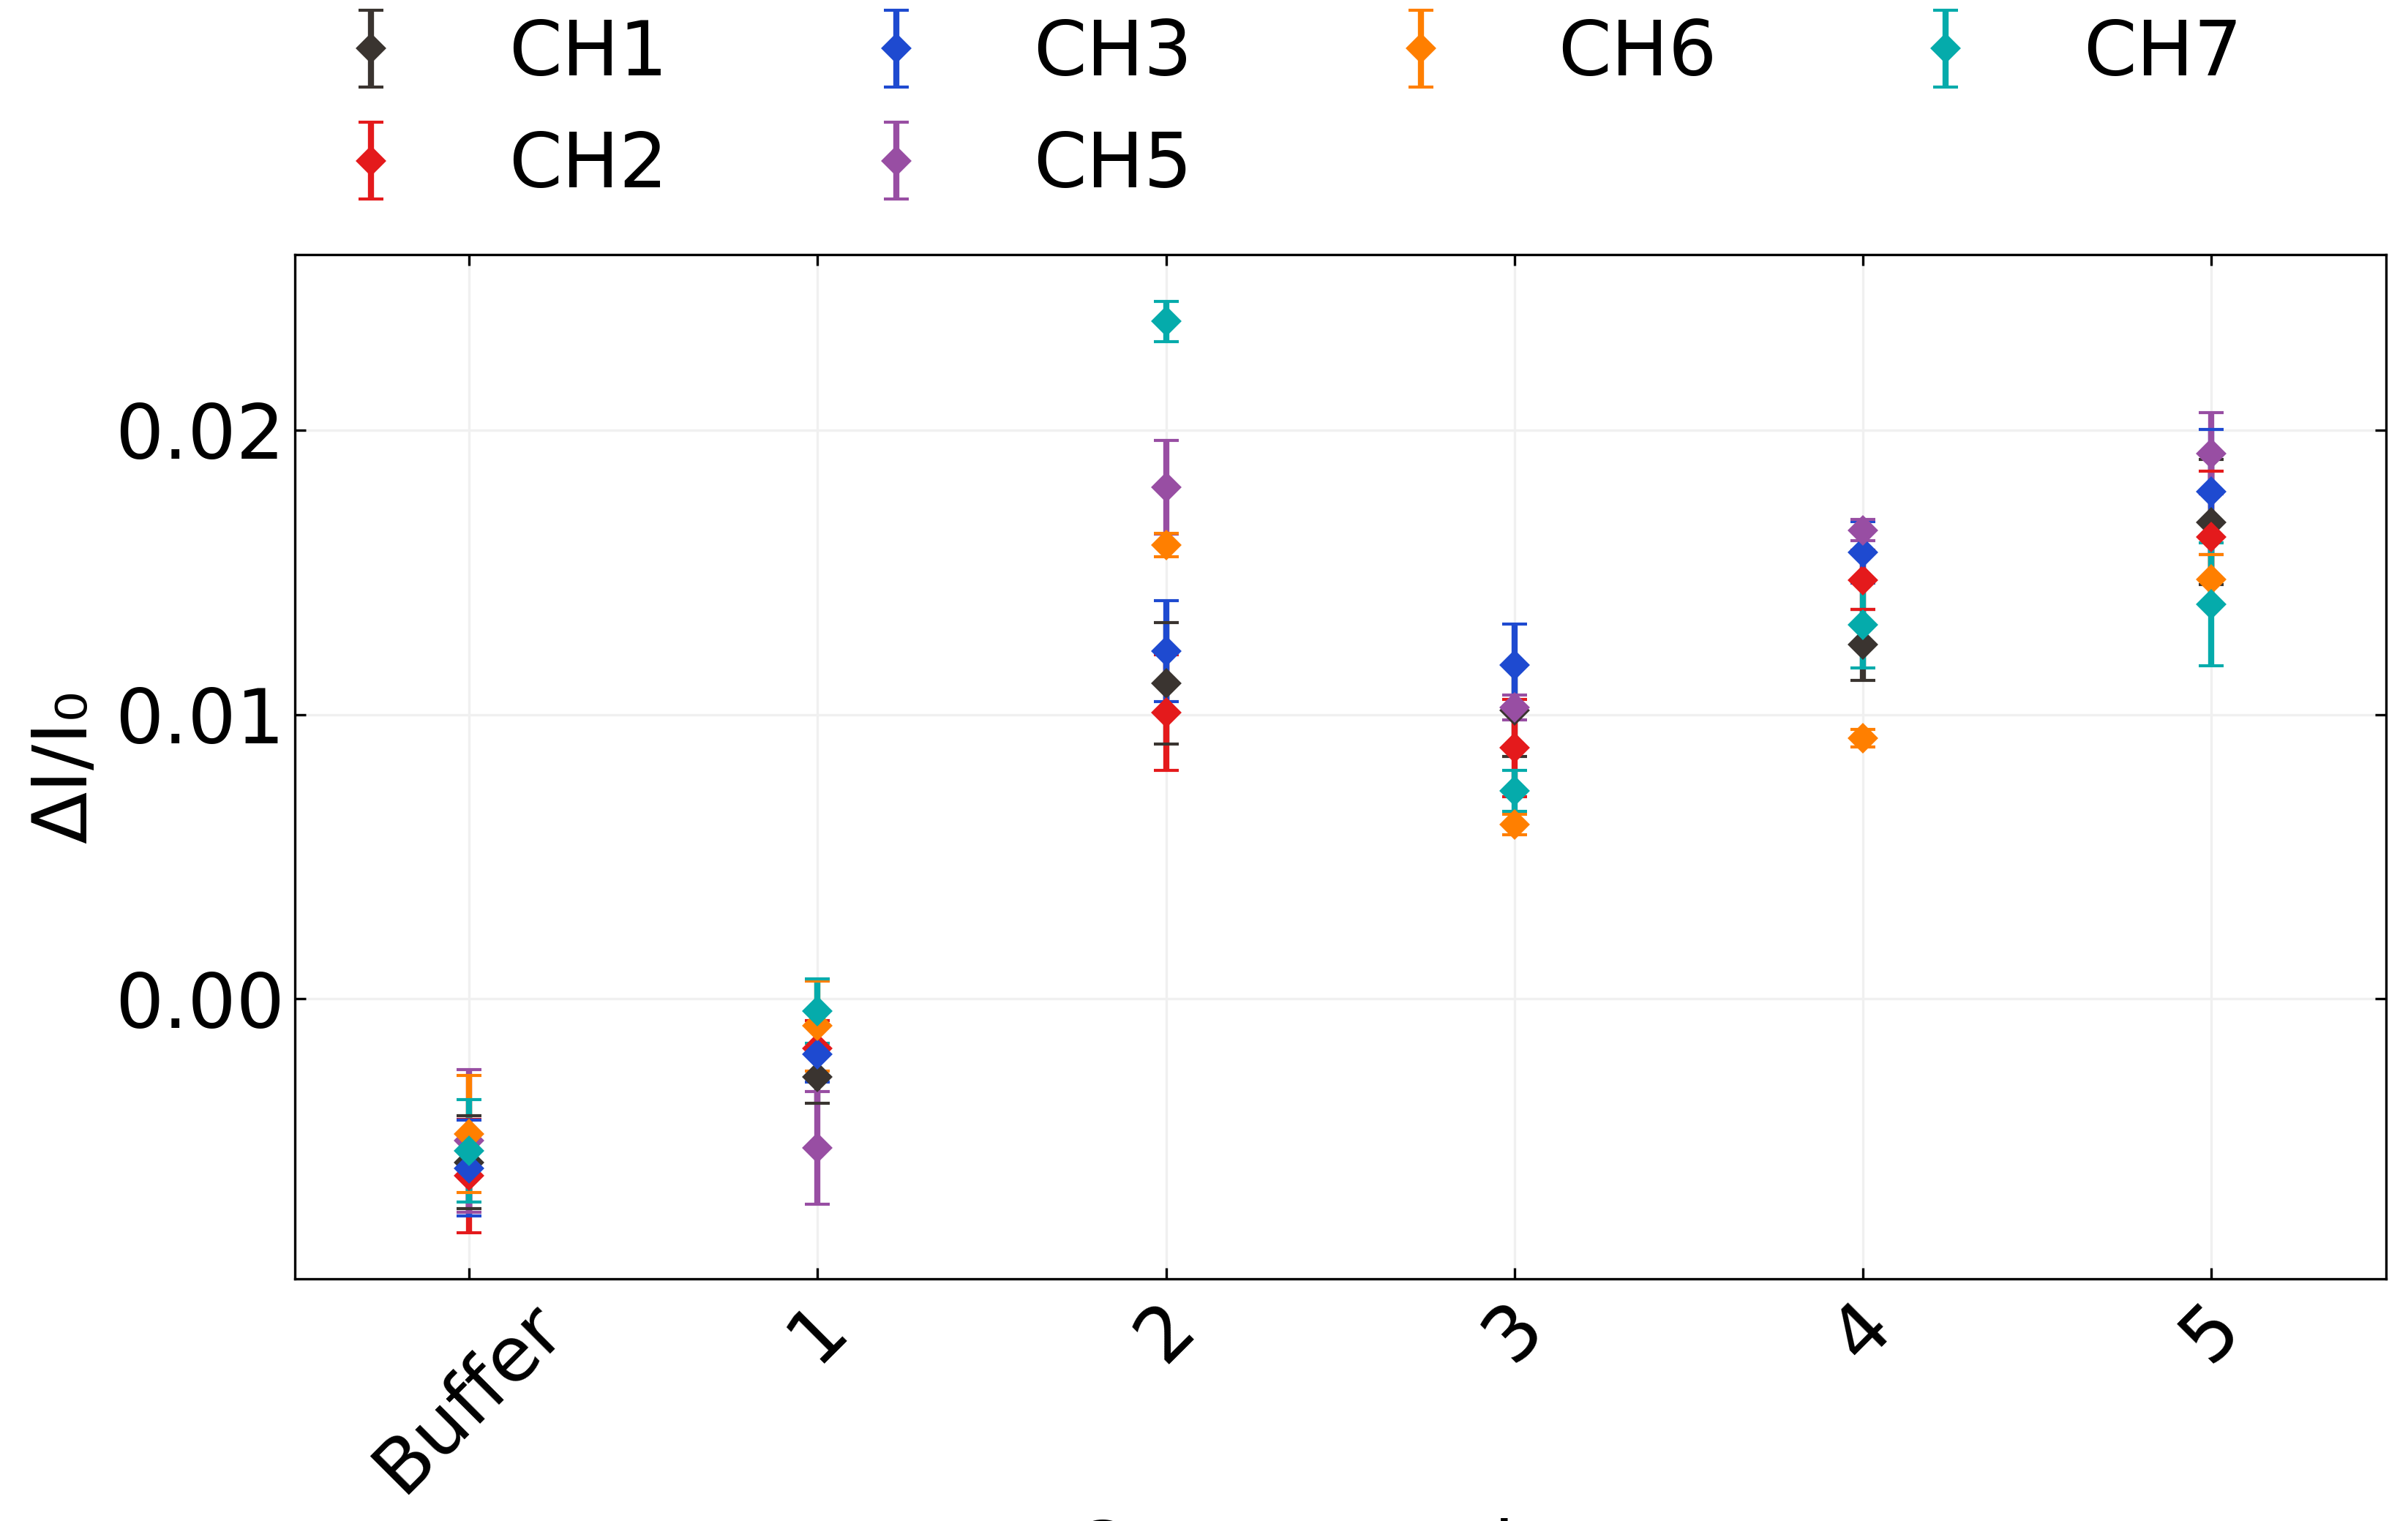
\includegraphics{./figures/app1/NTQ31C1_mean_simple_difference_before_and_after_step_filtered_concentrations.png}

}

}

\subcaption{\label{fig-spaa-no-detrend}}
\end{minipage}%
%
\begin{minipage}[t]{0.50\linewidth}

{\centering 

\raisebox{-\height}{

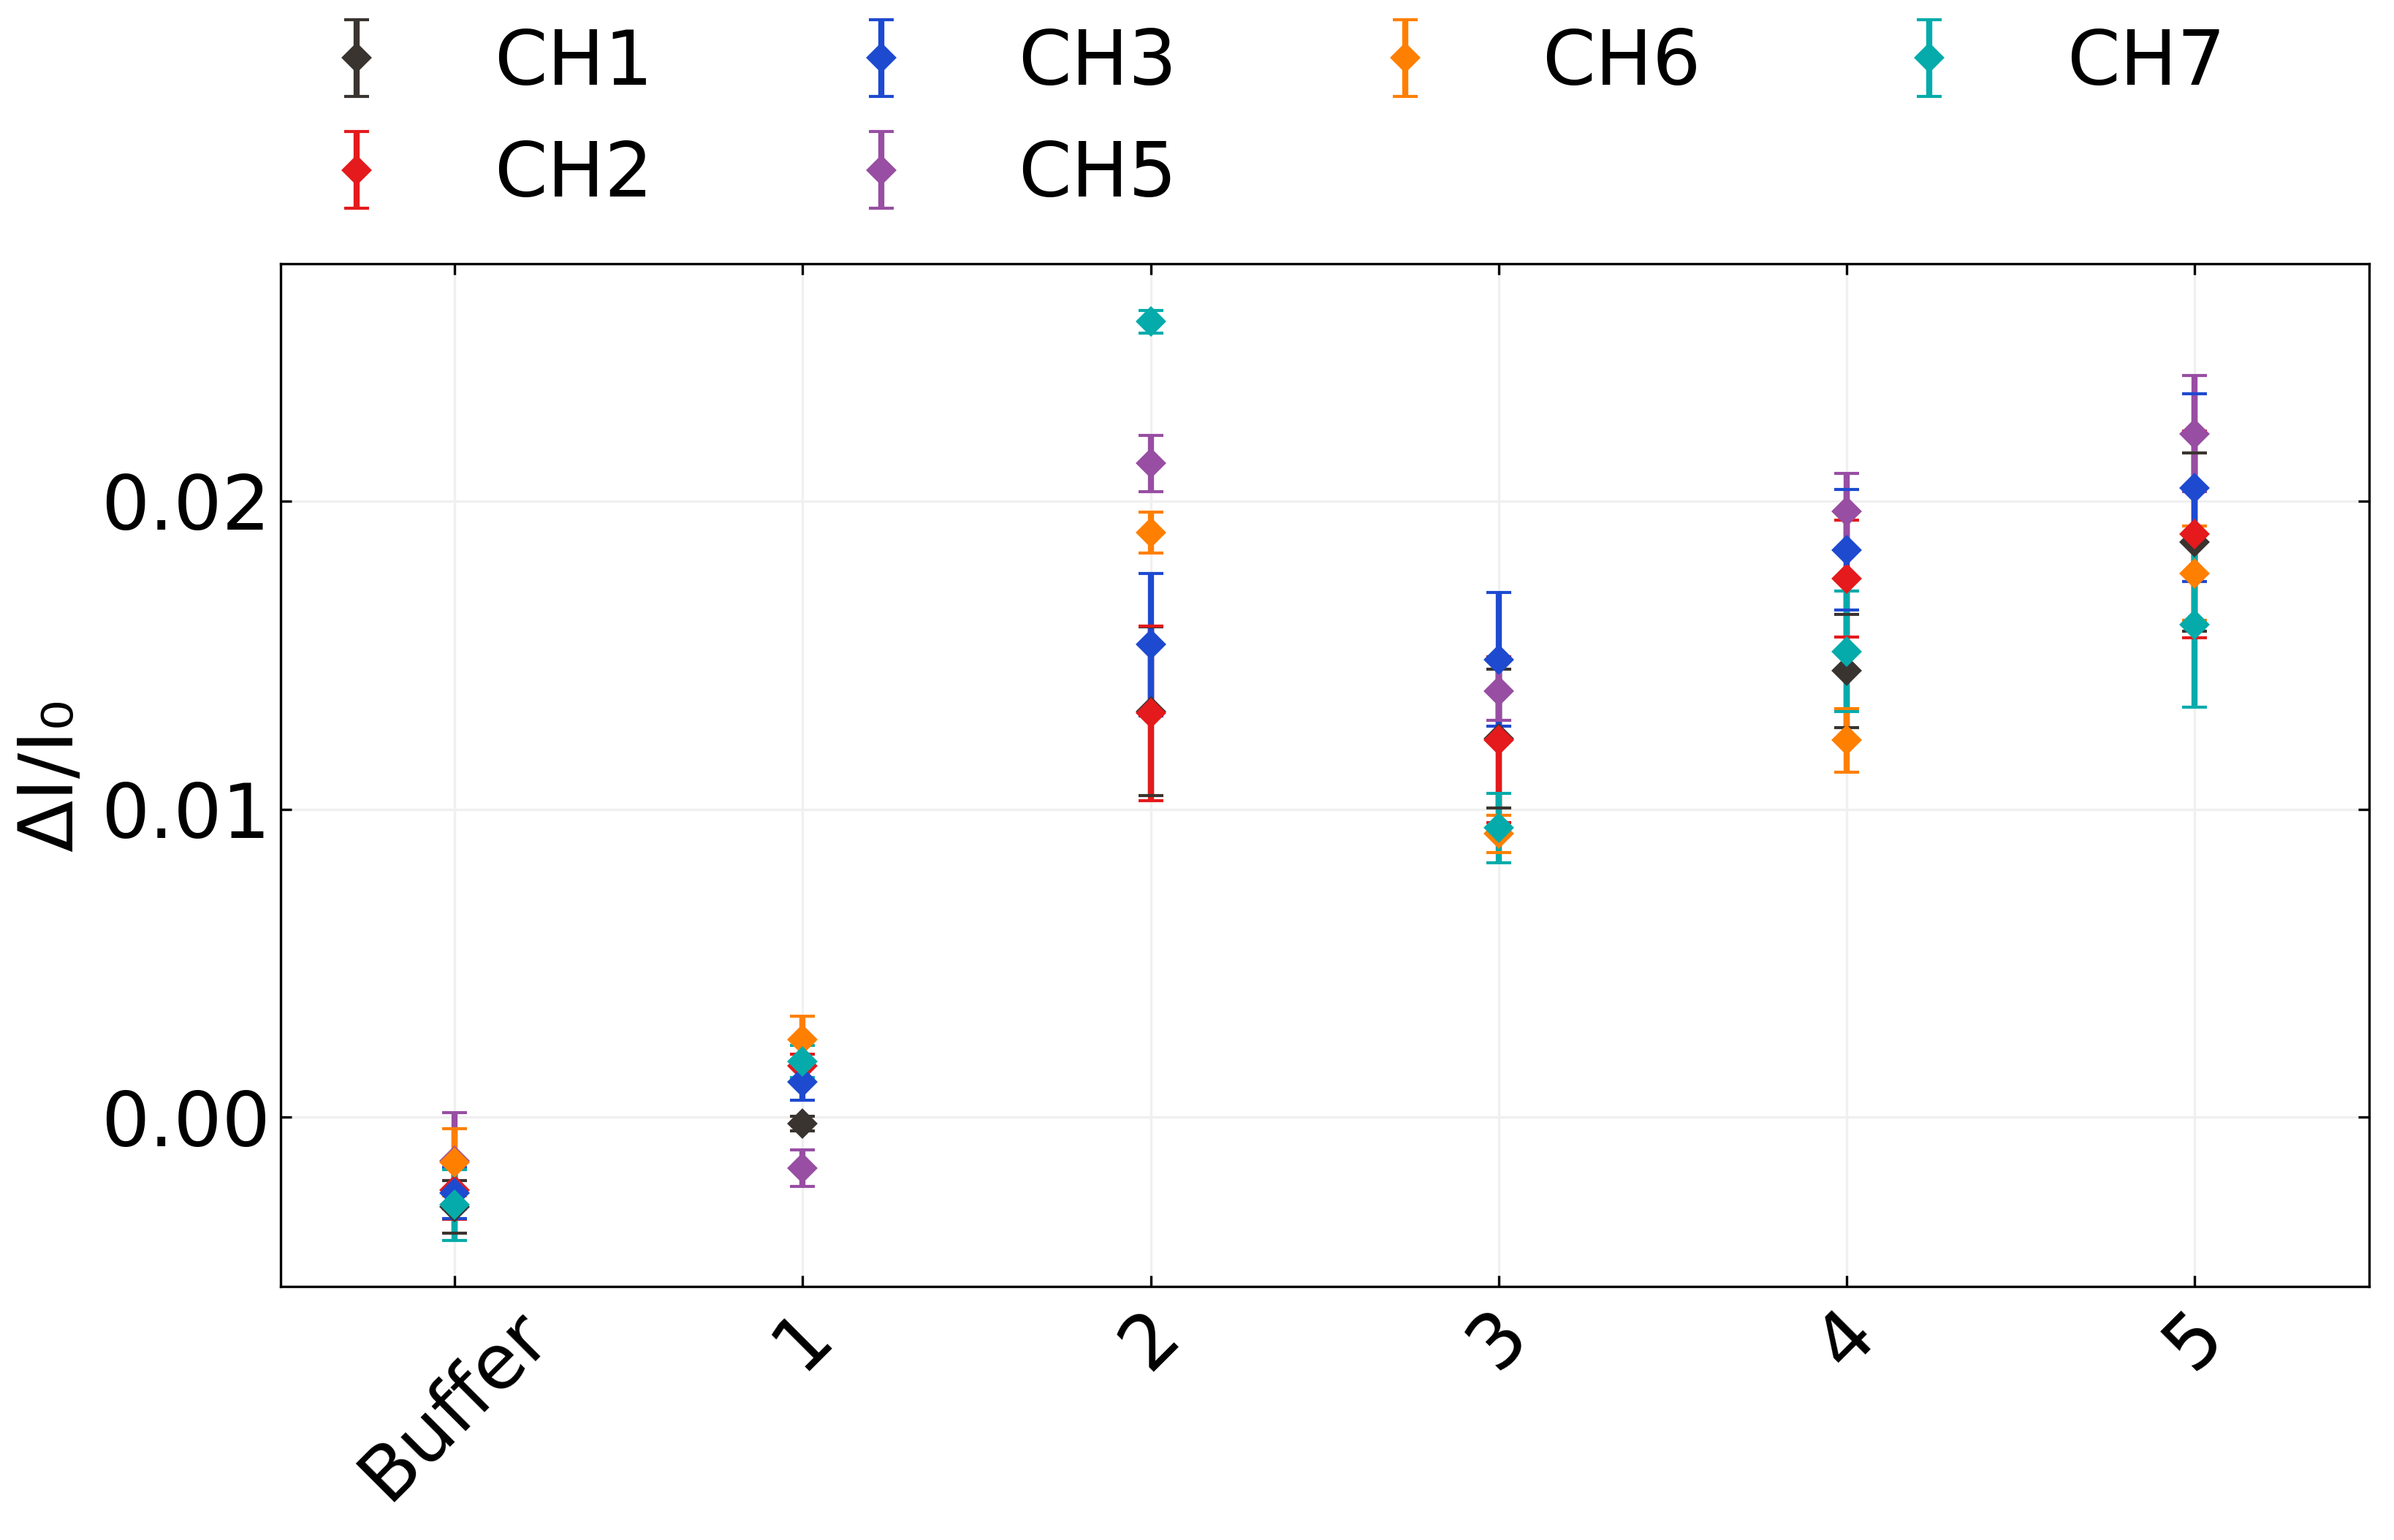
\includegraphics{./figures/app1/NTQ31C1_mean_simple_difference_before_and_after_step_filtered_concentrations_detrend.png}

}

}

\subcaption{\label{fig-spaa-detrend}}
\end{minipage}%

\caption{\label{fig-spaa-plot-comparison}A comparison of signal with
analyte addition plots taken from the same salt concentration sensing
dataset (the same dataset as used in \textbf{?@fig-salt-conc-sensing}).
In (a), a simple difference calculation performed on filtered data was
used, while in (b) the same calculation was performed on filtered data
with the baseline drift removed, the method used in the body of the
thesis.}

\end{figure}

The second module imports transfer measurements in .csv format and
creates combined and individual plots of the eight channels on a single
device. In combined plots, channels which are non-working, due to being
shorted or non-conducting, are removed via setting a maximum and minimum
possible on-current in the config file. Various parameters from the
transfer characteristics are saved as a spreadsheet along with standard
error. These parameters include on current, off current, subthreshold
slope and threshold voltage for the carbon nanotube devices, and on
current, off current and major Dirac point voltage for graphene devices.
The device type being analysed can be set in the config file.

The third module imports several transfer measurements in .csv format
and allows for comparison of the same channel before and after some
modification. It also calculates the shift in either threshold voltage
or major Dirac voltage of the device.

\hypertarget{vapour-delivery-system}{%
\chapter{Vapour Delivery System}\label{vapour-delivery-system}}

\hypertarget{technical-notes}{%
\section{Technical Notes}\label{technical-notes}}

Two LabView Virtual Instruments (VIs) were adapted from pre-existing VIs
for operating the mass flow controllers and monitoring vapour flow into
the device chamber, as well as monitoring temperature and humidity in
the vapour delivery system's manifold. These VIs were named ``\,'' A
third VI was developed in parallel which combined the first two Virtual
Instruments, alongside allowing the sequence of values to control the
mass flow controllers.

From Honours report: ``\,``\,'' Figure 12 gives the right side of the
front panel of the LabView VI sample with vapour.VI, which letsus preset
an autonomously-performed vapour sensing sequence. Each row in each
array module corresponds to a differennest step in this sequence. The
`howManySteps' module lets us set how many of these steps are performed.
The `Durations Array' module determines the length of time in seconds
each step is performed over. The `Carrier Flows Array' and `Dilution
Flows Array' modules let us set the carrier flow and dilution flow,
respectively, in standard cubic centimetres per minute (sccm) through
the gas rig at each step. The carrier flow pushes analyte vapour into
the vapour-sensing device chamber, while dilution flow is used to modify
the flow behaviour of the analyte vapour entering the chamber. The
vapour sensing sequence as depicted in Figure 12 was used for all vapour
sensing runs in this investigation. At the end of the sequence, the data
collected about the vapour sensing process was saved as an .lvm file.
``\,``\,''

\hypertarget{future-improvements}{%
\section{Future Improvements}\label{future-improvements}}


\backmatter
\printbibliography


\end{document}
